\documentclass[11pt]{article}
\usepackage[margin=1in]{geometry}
\usepackage{amsmath,amssymb,amsthm,mathtools}
\usepackage{booktabs,array}
\usepackage{microtype}
\usepackage[hidelinks,pdftitle={Factorizable Rational Quantum Channels at an Explicit Distance from Finite Tracial Baths},pdfauthor={Nidhal Mghirbi and Seth Douglas}]{hyperref}
\usepackage{enumitem}
\usepackage{xcolor}
\usepackage{tikz}
\usetikzlibrary{arrows.meta,positioning}
\usepackage{url}
\def\UrlBreaks{\do\_\do\.\do\/}
\raggedbottom

\definecolor{accent}{RGB}{22,102,113}
\definecolor{accentlight}{RGB}{231,242,244}
\definecolor{softgray}{RGB}{245,246,247}

\newtheorem{theorem}{Theorem}[section]
\newtheorem{lemma}[theorem]{Lemma}
\newtheorem{proposition}[theorem]{Proposition}
\newtheorem{corollary}[theorem]{Corollary}
\newtheorem{definition}[theorem]{Definition}
\newtheorem{remark}[theorem]{Remark}
\newtheorem{headline}{Theorem}
\renewcommand{\theheadline}{\Roman{headline}}
\newcommand{\tr}{\operatorname{tr}}
\newcommand{\Tr}{\operatorname{Tr}}
\newcommand{\Fact}{\operatorname{Fact}}
\newcommand{\K}{\mathcal K}
\newcommand{\N}{\mathcal N}
\newcommand{\eps}{\varepsilon}
\newcommand{\cJ}{\mathfrak J}
\newcommand{\Ad}{\operatorname{Ad}}
\newcommand{\ket}[1]{\lvert #1\rangle}
\newcommand{\bra}[1]{\langle #1\rvert}

\title{Factorizable Rational Quantum Channels at an Explicit Distance from Finite Tracial Baths}
\author{Nidhal Mghirbi \and Seth Douglas}
\date{October 2026}

\begin{document}
\maketitle
\begin{abstract}
A quantum channel can always be implemented by a unitary interaction with an environment that starts in a pure state.  With a finite, maximally mixed environment, the implementable channels are the noisy operations.  A tracial von Neumann algebra as environment gives the factorizable channels.  By a theorem of Haagerup and Musat, combined with $\mathrm{MIP}^*=\mathrm{RE}$, some of these lie outside the closure of the noisy operations.  In earlier work we wrote down explicit rational channels of this kind, with no value for their distance from the closure.  Using Wang and Zhi's dimension-uniform reflection estimate, we construct a factorizable unital channel on twelve qubits with Kraus entries in $\{0,1,\pm3/5,4/5\}$.  Its normalized Choi and diamond distances from the closure are at least $2^{-(2\cJ+50)}$, with $\cJ=2^{2^{1122000}}$.  The bound comes from a compiler theorem: group relations that are rigid uniformly in the matrix dimension give a rational channel with an explicit distance bound.  Unlike the bound of our earlier work, it needs reference positions only for the identity, the generators and their inverses.  For the earlier channels, a new spectral certificate for the root groups of their presentation, with Wang and Zhi's estimates, gives an explicit tolerance.  The fifteen-qubit channel and its two variants are then at distance at least $2^{-(2\cJ+41)}$ in both metrics.  By our earlier bound, the fourth channel, with a reference position for every group element it uses, is at Choi distance at least $2^{-(2\cJ+36)}$ and diamond distance at least $2^{-(2\cJ+21)}$.  These numbers are tiny because Wang and Zhi's tolerance is $2^{-\cJ}$.  Their method builds on the group construction of Kun and Thom and on nonhyperlinearity results of Thom, Liu, and Alekseev, Liu and Thom.  The finite certificates are checked by exact computation.
\end{abstract}

\section{Introduction}\label{sec:intro}

\subsection{The question}
Stinespring's theorem implements every quantum channel by a unitary interaction with an environment that starts in a pure state \cite{Stinespring55}.  Suppose instead that the environment must start maximally mixed, so that it supplies no purity.  The channels implementable this way, with a finite environment, are the \emph{noisy operations} of Horodecki, Horodecki and Oppenheim \cite{HHO03}.  Which channels are limits of noisy operations?

Every noisy operation is \emph{factorizable}: it factors through a finite von Neumann algebra with a faithful normal tracial state \cite[Definition~6.2]{Anantharaman06}, \cite[Theorem~2.2]{HaagerupMusat11}.  The factorizable channels form a closed set \cite[Remark~1.4(b) and proof of Theorem~6.1]{HaagerupMusat11}.  So every limit of noisy operations is unital and factorizable.  The ultraproduct argument in the proof of \cite[Theorem~3.6]{HaagerupMusat15} shows more: such a limit factors through an ultrapower of the hyperfinite $\mathrm{II}_1$ factor.  Haagerup and Musat showed that the converse, for all channels on all matrix algebras, is equivalent to a positive answer to Connes' embedding problem \cite[Theorem~3.7]{HaagerupMusat15}.  Since $\mathrm{MIP}^*=\mathrm{RE}$ \cite{JiEtAl20}, the converse fails: some factorizable channels are not limits of noisy operations.  That argument does not produce a channel one can write down.  The standard route from a non-embeddable algebra to such a channel goes through Schur multipliers and Kirchberg's unitary correlation matrices, in the form of Dykema and Juschenko \cite{Kirchberg93}, \cite{DykemaJuschenko11}, \cite[proof of Theorem~3.7]{HaagerupMusat15}, \cite[Corollary~3.11]{Musat25}.  Musat and R\o rdam showed that the limits of noisy operations are exactly the channels given by hyperlinear traces on the free product $M_d*_{\mathbb C}M_d$ \cite[Proposition~3.2(ii) and Theorem~2.10]{MusatRordam21}.  Neither route gives a channel or a distance without an explicit non-embeddable input.

Explicit examples nearby lie on either side of the question.  Nonfactorizable channels have no tracial realization at all \cite{HaagerupMusat11}; Haagerup and Musat showed that every nonfactorizable unital channel violates the asymptotic quantum Birkhoff conjecture, and that such channels exist on $M_n$ for every $n\ge3$ \cite[Theorem~6.1 and its proof]{HaagerupMusat11}.  For the Werner--Holevo channel $W_3^-$ they computed the cb distance to the factorizable channels exactly: it is $4/27$ \cite[Theorem~5.6(2)]{HaagerupMusat15}.  Channels that need an infinite-dimensional, indeed type~$\mathrm{II}_1$, ancilla can still be approximated by noisy operations \cite[Theorem~4.1]{MusatRordam20}; Mori's non-closure theorem for correlation matrices of unitaries \cite[Theorem~2.3]{Mori24} lowers the dimension of such examples from $11$ to $8$ \cite[Corollary~3.10]{Musat25}.  The channels of this paper are factorizable and lie at an explicit distance from the limits of noisy operations.

\subsection{Explicit channels}
In earlier work \cite{MghirbiDouglasV1} we wrote such channels down.  We built a finite presentation of a nonhyperlinear group modelled on a Kun--Thom pair over $\mathbb F_5$ \cite{KunThom26}.  It has a witness word that every homomorphism into a tracial ultraproduct of matrix algebras must kill.  This follows from Thom's normalization theorem and his witness argument \cite[Theorem~1.2 and Section~5.2]{Thom26}, with the internality theorem of Liu \cite[Theorem~1.2]{Liu26} in the form of Alekseev, Liu and Thom \cite[Theorem~B]{AlekseevLiuThom26}.  Rational $2\times2$ blocks turned the presentation into unital channels that are factorizable but not limits of noisy operations.  Each basis position of such a channel lies either in a $2\times2$ block, which encodes one relation $xy=z$ among group elements, or in a \emph{singleton} carrying one group element.  The group elements that occur are the \emph{labels}.  There were four channels.  The fully referenced channel $\Phi_{\rm full}$ on $M_{44086}$ ($\Phi_{\rm ref}$ in \cite{MghirbiDouglasV1}) has a singleton for every label.  The reduced channels are $\Phi_1$ on $M_{31981}$, with a singleton only for the identity; $\Phi_2$ on $M_{31982}$, with singletons for the identity and the witness; and $\Phi_{15}$, which pads $\Phi_2$ to fifteen qubits with $786$ further identity positions.  The subscripts of $\Phi_1$ and $\Phi_2$ count singleton labels, not qubits.  Their distances from the closure were shown to be positive, by an argument that rests on the preprints of Thom and of Alekseev, Liu and Thom, but no lower bound was given.  A compactness argument gives a tolerance $e_0$ on the relator defects that forces the witness close to the identity, but no value for $e_0$.  The same work converted any value of $e_0$ into explicit bounds for $\Phi_{\rm full}$ (Lemma~\ref{lem:fullref} below).  It noted that a quantitative support-leakage theorem would do the same for the reduced channels.

The group theory behind these constructions is recent.  Building on Kun's expander decomposition for Kazhdan groups \cite[Theorem~1]{Kun16}, OpenAI constructed the first nonsofic group \cite{OpenAI26}.  Kun and Thom then showed that amalgamated doubles of suitable Kazhdan pairs are nonsofic \cite[Theorems~A and~4.1]{KunThom26}, and gave explicit pairs over every finite field \cite[Theorem~E]{KunThom26}.  Alekseev and Thom proved that centralizers of sofic approximations of Kazhdan groups are internal \cite[Theorem~3.1]{AlekseevThom26}, and asked for the matrix analogue \cite[Open Problem~6.2(a)]{AlekseevThom26}.  Thom showed that a positive answer makes these doubles nonhyperlinear, with an explicit witness commutator \cite[Theorems~1.2 and~1.3 and Section~5.2]{Thom26}.  Liu answered the problem positively \cite[Theorem~1.2]{Liu26} and proved that a Kun--Thom wreath product is not hyperlinear \cite[Theorem~1.1]{Liu26}.  Alekseev, Liu and Thom proved a stronger internality theorem, for unitary tuples with spectral gap \cite[Theorem~B]{AlekseevLiuThom26}, and deduced that the doubles are not hyperlinear \cite[Corollary~C]{AlekseevLiuThom26}.

Forcing operator relations through channels or correlations has precedents.  Musat and R\o rdam prescribe a correlation matrix of unitaries that forces projections to sum to an irrational multiple of the identity, and obtain a Schur-multiplier channel that needs a type~$\mathrm{II}_1$ ancilla \cite[Theorem~4.1]{MusatRordam20}.  Mori forces a product relation among symmetries through unitary correlation matrices \cite{Mori24}.  Slofstra embeds group relations in nonlocal games \cite{Slofstra20}, and Paulsen and Rahaman obtain factorizable maps from bisynchronous game correlations \cite{PaulsenRahaman21}.

\subsection{Main results}
Wang and Zhi have recently made this forced triviality quantitative \cite{WangZhi26}, with explicit forms of the spectral correction of Alekseev, Liu and Thom and of Thom's normalization theorem.  Their reflection estimate holds uniformly in the matrix dimension.  It concerns their auxiliary relation system, a finite set of group relations; Appendix~\ref{app:relations} gives the form we use.  Represent the root symbols by exact symmetries, and let every relation defect be below $2^{-\cJ-7}$, where $\cJ=2^{2^{1122000}}$.  Then two fixed conjugates of a root element lie within $5\cdot2^{-20}$ of each other \cite[Theorem~5.2]{WangZhi26} (Theorem~\ref{thm:reflection}).  They use it to give an explicit polynomial counterexample to the algebraic form of Connes' embedding conjecture.  We use it, and their method, to give explicit channels.  Their paper, and the preprints of Thom and of Alekseev, Liu and Thom that its proofs use, are not yet refereed.  Section~\ref{sec:new} lists which of our results depend on them.  From Kun and Thom's preprint we use only the groups.

Write $\N_d$ for the noisy operations on $M_d$, $\K_d$ for their closure, and $\Delta_J$ and $\Delta_\diamond$ for the normalized Choi and diamond distances to $\K_d$ (Section~\ref{sec:setup}).  An explicit positive lower bound on $\Delta_J$ or $\Delta_\diamond$ is called a \emph{gap} below.

\begin{headline}[Section~\ref{sec:12q}]\label{hl:12q}
There is an explicit unital channel $\Phi_{12}$ on $M_{4096}$, factorizable through the group von Neumann algebra of the amalgamated double of a Kun--Thom pair over $\mathbb F_8$ used by Wang and Zhi, with Kraus entries in $\{0,1,\pm3/5,4/5\}$ and Choi rank $949$, such that
\[
 \Delta_J(\Phi_{12})\ge2^{-(2\cJ+50)},\qquad\Delta_\diamond(\Phi_{12})\ge2^{-(2\cJ+50)}.
\]
\end{headline}

\begin{headline}[Theorem~\ref{thm:gap}]\label{hl:compiler}
Take a finite relation system with relators of length at most six, and a tracial group model in which two generators $p$ and $q$ are distinct.  Compile it into a rational channel $\Phi$ on $M_d$ (Definition~\ref{def:compiler}): one block for each prefix multiplication of each relator and for each generator inverse, and one singleton position for the identity and for each distinct value of a generator or inverse.  Further singletons are allowed.  Suppose that for some $0<\rho_0\le2$, in every matrix dimension, every unitary assignment with all relator defects $\|v(R)-I\|_2$ at most $\rho_0$ has $\|v_p-v_q\|_2\le\tfrac12$.  Then $\Phi$ is factorizable, as in \cite[Proposition~3]{MghirbiDouglasV1}, and $\Delta_J(\Phi),\Delta_\diamond(\Phi)\ge(\rho_0/512)^2/d$.
\end{headline}

\begin{headline}[Section~\ref{sec:old15}]\label{hl:v1}
For the channels of \cite{MghirbiDouglasV1}, each reduced channel $\Phi\in\{\Phi_1,\Phi_2,\Phi_{15}\}$ satisfies $\Delta_J(\Phi),\Delta_\diamond(\Phi)\ge2^{-(2\cJ+41)}$.  The fully referenced channel satisfies $\Delta_J(\Phi_{\rm full})\ge2^{-(2\cJ+36)}$ and $\Delta_\diamond(\Phi_{\rm full})\ge2^{-(2\cJ+21)}$, by the bound of \cite[Theorem~6]{MghirbiDouglasV1} (Lemma~\ref{lem:fullref}) with the tolerance of Theorem~\ref{thm:f5rigidity}.
\end{headline}

Theorem~\ref{hl:v1} gives explicit gaps for all four earlier channels.  $\Phi_{12}$ acts on fewer qubits than any of them, but its gap is $2^9$ times smaller than that of $\Phi_{15}$.  The two come from different relation systems, and neither bound is claimed to be optimal.  The rigidity input of Theorem~\ref{hl:v1} is a new spectral certificate for the characteristic-five root groups of the $43$-generator presentation (Appendix~\ref{sec:f5rigidity}).  Theorem~\ref{thm:f5rigidity} runs Wang and Zhi's proof of their reflection estimate \cite[Theorem~5.2]{WangZhi26} on this presentation, with their explicit forms of the spectral correction of Alekseev, Liu and Thom and of Thom's normalization \cite[Corollary~4.3 and Theorem~4.1]{WangZhi26}.  The proof for the reduced channels uses a leakage theorem that needs no singletons for the generators (Theorem~\ref{thm:oldleak}), a quantitative form of \cite[Lemma~2]{MghirbiDouglasV1}, and the Kraus-vector coherence test of \cite[Theorem~5]{MghirbiDouglasV1}.  Table~\ref{tab:positioning} places these results among the known separations.

Two further points.  For $\Phi_{12}$ and for the earlier reduced channels, one fixed two-outcome measurement on the Choi state separates the channel from all of $\K_d$ (Corollary~\ref{cor:witness} and the remark after it).  At errors below the gap, the gaps force linear purity consumption in repeated use.  They also force linear memory when the exchanged qubits are capped (Section~\ref{sec:memory} for $\Phi_{12}$; the end of Section~\ref{sec:old15} for $\Phi_2$ and $\Phi_{15}$).  The constants are astronomically small, inherited from the tolerance $2^{-\cJ}$.  They replace a compactness argument by an explicit bound; they do not describe an experiment.

\begin{table}[b]
\centering
\small
\begin{tabular}{@{}>{\raggedright\arraybackslash}p{0.2\textwidth}>{\raggedright\arraybackslash}p{0.26\textwidth}>{\raggedright\arraybackslash}p{0.26\textwidth}>{\raggedright\arraybackslash}p{0.2\textwidth}@{}}
\toprule
 & explicit object & separation & rigidity input\\
\midrule
$\mathrm{MIP}^*=\mathrm{RE}$ \cite{JiEtAl20} & none & existence & ---\\
Liu \cite{Liu26}; Alekseev--Liu--Thom \cite{AlekseevLiuThom26} & nonhyperlinear groups & witness forced trivial; no value & internality; Thom's normalization\\
Mghirbi--Douglas \cite{MghirbiDouglasV1} & rational channels, dimensions $31981$ to $44086$ & positive, no value & Alekseev--Liu--Thom, Thom\\
Wang--Zhi \cite{WangZhi26} & degree-$12$ polynomial, $65$ variables & $\tr f\ge3/4$ vs.\ $-1$ & explicit forms of Alekseev--Liu--Thom and Thom\\
This paper & a 12-qubit channel, and the channels of \cite{MghirbiDouglasV1} & explicit: $2^{-(2\cJ+50)}$; $2^{-(2\cJ+41)}$ and $2^{-(2\cJ+36)}$ & Wang--Zhi; new certificate\\
\bottomrule
\end{tabular}
\caption{Known failures of Connes' embedding, from existence to explicit polynomials and channels.  The gap $2^{-(2\cJ+41)}$ holds for $\Phi_1$, $\Phi_2$ and $\Phi_{15}$; the Choi-distance gap of $\Phi_{\rm full}$ is listed last.}
\label{tab:positioning}
\end{table}

\subsection{What is new and what is not}\label{sec:new}
The rational block of Figure~\ref{fig:block} and the principle that a nearby finite-bath channel yields an approximate representation of the relations are from \cite{MghirbiDouglasV1}, in exact form \cite[Lemma~2 and Proposition~3]{MghirbiDouglasV1} and in quantitative form for fully referenced channels \cite[Theorems~6 and~I.1]{MghirbiDouglasV1}.  So are the coherence tests, between two singleton positions and between two Kraus vectors \cite[Theorems~5 and~I.1]{MghirbiDouglasV1}.  The singleton test is a quantitative form of the Haagerup--Musat criterion for Schur channels \cite[Proposition~2.8]{HaagerupMusat11} (Lemma~2.8 in the arXiv version).  For a Schur channel, the unitary of an exact factorization is block diagonal, and its diagonal blocks are unitaries whose correlation matrix is the Schur matrix.  With Wang and Zhi's tolerance, the argument of Lemma~\ref{lem:fullref}, with the two signal singletons in place of the identity and the witness, would already give an explicit gap for a fully referenced channel of their relation system, on thirteen qubits (Remark~\ref{rem:13q}).  The compiler of Section~\ref{sec:compiler} needs singletons only for the identity and the \emph{letters}, the generators and their inverses, and recovers the relations from the multiplication blocks.  This brings the channel to twelve qubits, with a diamond bound weaker by a factor of about $2^{13}$.  The new mathematics here is that compiler (Theorems~\ref{thm:extract} and~\ref{thm:gap}), the leakage theorem without letter singletons (Theorem~\ref{thm:oldleak}), and the characteristic-five root certificate (Appendix~\ref{sec:f5rigidity}); Theorem~\ref{thm:f5rigidity} is Wang and Zhi's argument run on that certificate.  The explicit witness follows in a few lines from the proof of the compiler.  The repeated-use bounds of Section~\ref{sec:memory} are applications of results from our companion papers.

\paragraph{Dependencies.}
\begin{itemize}
\item No recent preprint is used in Theorems~\ref{thm:extract} and~\ref{thm:gap} (hence Theorem~\ref{hl:compiler}), Lemma~\ref{lem:anchor}, Corollary~\ref{cor:witness}, Theorem~\ref{thm:oldleak}, Lemma~\ref{lem:fullref}, Proposition~\ref{prop:finite-system}, the certificate~\eqref{eq:integer-residual}, Lemmas~\ref{lem:f5pairspectrum} and~\ref{lem:f5collection} and Proposition~\ref{prop:f5rootres}.
\item Proposition~\ref{prop:rho}, Theorems~\ref{thm:12q}, \ref{thm:oldglobal} and~\ref{thm:f5rigidity}, and Corollary~\ref{cor:full} use Wang and Zhi's theorems, and through them steps of Thom and of Alekseev, Liu and Thom.  So do Theorems~\ref{hl:12q} and~\ref{hl:v1}, the explicit witness margins of Section~\ref{sec:witness}, Corollary~\ref{cor:memory}, the repeated-use statements at the end of Section~\ref{sec:old15} and Remark~\ref{rem:13q}.  These results depend on preprints that are not yet refereed.
\item Lemma~\ref{lem:wz-tolerance} uses only Wang and Zhi's parameter recipe and the arithmetic in their proof of Lemma~5.1.
\item No result uses a theorem of Kun and Thom: we use their groups, and the facts we need about them are checked by exact computation.
\item Corollary~\ref{cor:memory} and the end of Section~\ref{sec:old15} also rest on our companion reports \cite{DouglasMghirbiCausal,DouglasMghirbiC} and on \cite[Proposition~K.3]{MghirbiDouglasV1}, which are not refereed either.
\item The bounds of Theorem~\ref{hl:v1} use the triangle table and Theorem~\ref{thm:f5rigidity}, not the group model of Section~\ref{sec:old15}.  The model gives factorizability; the scripts of Section~\ref{sec:repro} check its finite facts.
\end{itemize}

\begin{figure}[t]
\centering
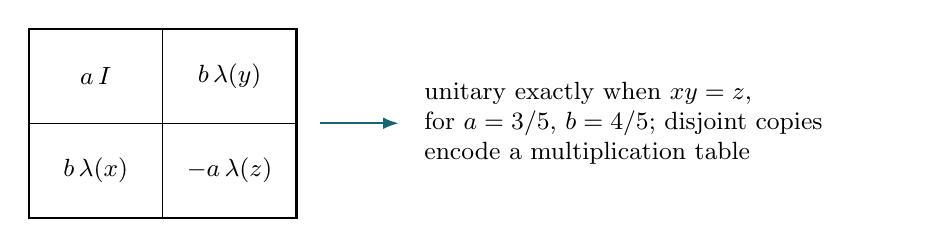
\begin{tikzpicture}[every node/.style={font=\small}]
  \draw[thick] (0,0) rectangle (3.4,2.4);
  \draw (1.7,0)--(1.7,2.4); \draw (0,1.2)--(3.4,1.2);
  \node at (0.85,1.8) {$a\,I$};
  \node at (2.55,1.8) {$b\,\lambda(y)$};
  \node at (0.85,0.6) {$b\,\lambda(x)$};
  \node at (2.55,0.6) {$-a\,\lambda(z)$};
  \draw[-{Latex[length=2mm]}, thick, accent] (3.7,1.2)--(4.7,1.2);
  \node[align=left, text width=6.2cm, anchor=west] at (4.9,1.2) {unitary exactly when $xy=z$,\\ for $a=3/5$, $b=4/5$; disjoint copies\\ encode a multiplication table};
\end{tikzpicture}
\caption{The rational block of \cite{MghirbiDouglasV1}.  It equals $\mathrm{diag}(I,\lambda(x))\bigl(\begin{psmallmatrix}a&b\\b&-a\end{psmallmatrix}\otimes I\bigr)\mathrm{diag}(I,\lambda(y))$ when $xy=z$.}
\label{fig:block}
\end{figure}

\subsection{Organization}
Section~\ref{sec:setup} fixes conventions.  Section~\ref{sec:compiler} proves the compiler theorems.  Section~\ref{sec:12q} applies them to Wang and Zhi's relation system, and Section~\ref{sec:witness} gives the explicit witness.  Section~\ref{sec:memory} records the repeated-use consequences.  Section~\ref{sec:old15} gives explicit gaps for the earlier channels.  Section~\ref{sec:repro} describes the verification scripts, and Section~\ref{sec:discussion} discusses open directions.  The appendices give the relation system (\ref{app:relations}), the spectral certificates (\ref{sec:spectral}), the statements we use from Wang and Zhi (\ref{sec:rigidity}), and the characteristic-five rigidity (\ref{sec:f5rigidity}).

\section{Setting}\label{sec:setup}

Let $M_d=M_d(\mathbb C)$, let $\tau_m=\Tr/m$ be the normalized trace on $M_m$, and write $\|X\|_2=\tau_m(X^*X)^{1/2}$ for the normalized Hilbert--Schmidt norm and $\|X\|$ for the operator norm.  A \emph{noisy operation} on $M_d$ is a channel of the form
\begin{equation}\label{eq:matrixtracial}
 \Psi(X)=(\mathrm{id}\otimes\tau_m)\bigl[U(X\otimes I_m)U^*\bigr],\qquad U\in U(dm),
\end{equation}
for some $m$.  Write $\N_d$ for this set and $\K_d$ for its closure.  These are the channels with an exact factorization through $M_d\otimes M_m$ \cite[Definition~3.1]{HaagerupMusat15}, the $m$-noisy channels of Musat's survey, which uses ``noisy operations'' for a larger class \cite{Musat25}.  The channels that factor through a finite-dimensional tracial von Neumann algebra are the finite convex mixtures of noisy operations, and they have the same closure \cite[Proposition~3.8(ii)]{Musat25}, so $\K_d$ does not depend on which finite baths are allowed.  A channel is \emph{factorizable} if it has the form~\eqref{eq:matrixtracial} with $(M_m,\tau_m)$ replaced by a finite von Neumann algebra with a faithful normal tracial state; the class was introduced by Anantharaman-Delaroche \cite[Definition~6.2]{Anantharaman06} and characterized in this unitary form by Haagerup and Musat \cite[Theorem~2.2]{HaagerupMusat11}.  Write $\Fact_d$ for this set.  By a theorem of Haagerup and Musat, $\K_d$ consists of the channels that admit a factorization through a finite von Neumann algebra that embeds trace-preservingly into an ultrapower of the hyperfinite $\mathrm{II}_1$ factor \cite[Theorem~3.6]{HaagerupMusat15}.  Such a channel can have other ancillas that do not embed.  So $\N_d\subseteq\K_d\subseteq\Fact_d$ (Figure~\ref{fig:classes}).  Equality $\K_d=\Fact_d$ for every $d$ is equivalent to a positive answer to Connes' embedding problem \cite[Theorem~3.7]{HaagerupMusat15}.

For $\ket{\Omega_d}=d^{-1/2}\sum_i\ket{i,i}$ let $J(\Phi)=(\Phi\otimes\mathrm{id})(\ket{\Omega_d}\!\bra{\Omega_d})$ be the normalized Choi state.  We use
\[
 d_J(\Phi,\Psi)=\tfrac12\|J(\Phi)-J(\Psi)\|_1,\qquad d_\diamond(\Phi,\Psi)=\tfrac12\|\Phi-\Psi\|_\diamond,
\]
and write $\Delta_J(\Phi)$ and $\Delta_\diamond(\Phi)$ for the distances from $\Phi$ to $\K_d$.  Since a maximally entangled input is admissible in the diamond norm, $d_J\le d_\diamond$.  Haagerup and Musat measure distance in the cb norm of maps on $M_d$.  By duality $\|\Phi-\Psi\|_\diamond=\|\Phi^*-\Psi^*\|_{\rm cb}$, where $\Phi^*$ is the Hilbert--Schmidt adjoint, and the adjoint of a noisy operation is a noisy operation, with $U^*$ in place of $U$.  So $\Delta_\diamond(\Phi)=\tfrac12\,\mathrm{dist}_{\rm cb}(\Phi^*,\K_d)$.  The Choi distance does not change when both channels are replaced by their adjoints, so also $\mathrm{dist}_{\rm cb}(\Phi,\K_d)\ge2\Delta_J(\Phi)$.  For example, Haagerup and Musat's cb distance $4/27$ from $W_3^-$ to the factorizable channels is a half-diamond distance of $2/27$.  This holds because $W_3^-$ is its own adjoint and adjoints of factorizable channels are factorizable \cite[Remark~1.4(b)]{HaagerupMusat11}.  The closure $\K_d$ is the same in every norm.  For an effect $0\le F\le I$ and two channels, $d_J(\Phi,\Psi)\ge|\Tr F(J(\Psi)-J(\Phi))|$.

\begin{figure}[t]
\centering
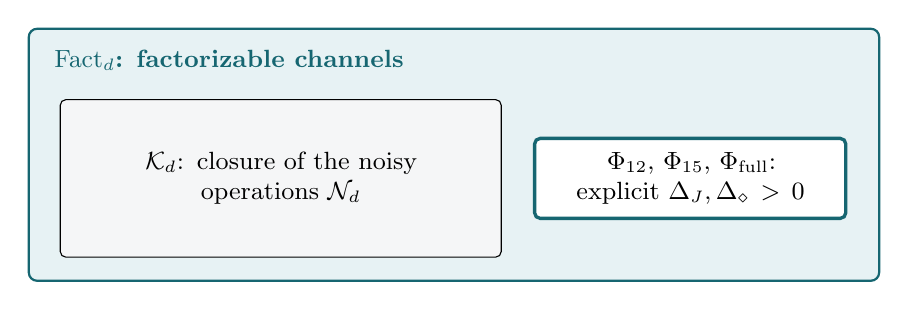
\begin{tikzpicture}[every node/.style={font=\small}]
  \draw[rounded corners=3pt, fill=accentlight, draw=accent, thick] (-5.4,-1.7) rectangle (5.4,1.5);
  \node[anchor=north west, text=accent, font=\small\bfseries] at (-5.2,1.35) {$\Fact_d$: factorizable channels};
  \draw[rounded corners=2pt, fill=softgray] (-5.0,-1.4) rectangle (0.6,0.6);
  \node[align=center, text width=5.2cm] at (-2.2,-0.4) {$\K_d$: closure of the noisy\\ operations $\N_d$};
  \node[draw=accent, very thick, rounded corners=2pt, fill=white, align=center, text width=3.6cm, inner sep=5pt] at (3.0,-0.4) {$\Phi_{12}$, $\Phi_{15}$, $\Phi_{\rm full}$:\\ explicit $\Delta_J,\Delta_\diamond>0$};
\end{tikzpicture}
\caption{The classes of Section~\ref{sec:setup}.  The channels of this paper are factorizable and, using the preprints listed in Section~\ref{sec:new}, at an explicit positive distance from $\K_d$.}
\label{fig:classes}
\end{figure}

\section{From relations to rational channels}\label{sec:compiler}

\subsection{The compiled channel}
A \emph{relation system} is a finite set of positive generators and a finite set $\mathcal R$ of relators, words in the generators and their inverses; we call the generators and their inverses \emph{letters}.  A \emph{tracial group model} is a homomorphism from the free group on the generators to a countable group $\Gamma$ that kills every relator; we use it with the trace $\tau$ of the group von Neumann algebra and write $\lambda$ for the left regular representation.  The \emph{labels} are the elements of $\Gamma$ that occur below: the identity, the values of all letters, and the values of all relator prefixes.  For example, take one generator $s$ and the relator $ss$, with $\Gamma=\mathbb Z/2$.  The relator has prefixes $s$ and $ss$, with labels $s$ and $1$; since $s=s^{-1}$ in $\Gamma$, the letters $s$ and $s^{-1}$ have the same label.  For a unitary assignment $s\mapsto v_s$ to the positive generators, the \emph{defect} of a relator $R$ is $\|v(R)-I\|_2$, where $v(R)$ evaluates $R$ with $v_{s^{-1}}=v_s^*$.

Each multiplication $xy=z$ among labels is encoded by a \emph{triangle}: the block of Figure~\ref{fig:block}, with $a=3/5$, $b=4/5$, on two system positions of its own.  For a generator $s$, the triangle $(s,s^{-1},1)$ is its \emph{inverse triangle}.

\begin{definition}[Anchored-letter compiler]\label{def:compiler}
The compiled channel has, on disjoint system positions,
\begin{enumerate}[label=(\roman*)]
\item a singleton position for the identity and one for every distinct letter label, and, optionally, singletons for further labels, each label having at most one singleton;
\item a triangle for every prefix multiplication of every relator, read left to right, and the inverse triangle of every generator; equal triangles are merged.
\end{enumerate}
At a singleton for label $g$ the Kraus operator $A_g$ has entry $1$.  On a triangle $(x,y,z)$ occupying positions $k,k+1$,
\[
 (A_1)_{kk}=a,\qquad (A_y)_{k,k+1}=b,\qquad (A_x)_{k+1,k}=b,\qquad (A_z)_{k+1,k+1}=-a.
\]
The channel is $\Phi(X)=\sum_gA_gXA_g^*$, the sum over labels.
\end{definition}

In the example, the only triangle is $(s,s,1)$, both a prefix triangle and the inverse triangle, and the compiled channel lives on four positions: singletons for $1$ and $s$, and one block.

The block of Figure~\ref{fig:block} is unitary because $a^2+b^2=1$ and $xy=z$, so $U_\Gamma=\sum_gA_g\otimes\lambda(g)$ is unitary on $\mathbb C^d\otimes\ell^2(\Gamma)$.  Distinct labels are distinct elements of $\Gamma$, so $\tau(\lambda(g)\lambda(h)^*)=\delta_{gh}$ and
\[
 (\mathrm{id}\otimes\tau)\bigl[U_\Gamma(X\otimes1)U_\Gamma^*\bigr]=\sum_gA_gXA_g^*=\Phi(X).
\]
Thus $\Phi$ is unital, trace preserving and factorizable, with Choi rank equal to the number of labels.  This is the block factorization of \cite[Proposition~3]{MghirbiDouglasV1}, an instance of the coefficient criterion of Haagerup and Musat \cite[Theorem~2.2]{HaagerupMusat11}, written in our convention $U(X\otimes1)U^*$.

\subsection{Extraction from small support leakage}
Let $\Pi$ be the support projection of $J(\Phi)$.  For a noisy operation $\Psi$ with unitary $U$ as in~\eqref{eq:matrixtracial}, write $U=\sum_{ij}\ket i\!\bra j\otimes U_{ij}$ with bath blocks $U_{ij}\in M_m$.  From the definitions,
\[
 J(\Psi)=\frac1d\sum_{i,j,k,l}\tau_m(U_{ij}U_{kl}^*)\,\ket i\!\bra k\otimes\ket j\!\bra l,
\]
the Gram matrix of the $d^2$ bath blocks in $L^2(M_m,\tau_m)$, divided by $d$.  Identify $\ket i\otimes\ket j$ with the matrix unit $E_{ij}$.  The Kraus matrices have pairwise disjoint supports, so they are orthogonal, and $\Pi$ is the projection onto their span.  Projecting $U$, as an element of $M_d\otimes L^2(M_m,\tau_m)$, onto $\mathrm{span}\{A_g\}\otimes L^2$ gives
\begin{equation}\label{eq:split}
 U=W+R,\qquad W=\sum_gA_g\otimes B_g,\qquad B_g=\frac{\sum_{ij}(A_g)_{ij}U_{ij}}{\sum_{ij}(A_g)_{ij}^2},
\end{equation}
and since the supports are disjoint, $W_{ij}=(A_g)_{ij}B_g$ for the one label $g$ whose Kraus matrix has entry $(i,j)$, and $W_{ij}=0$ if there is none.  For an exact factorization $R=0$ and the $B_g$ are orthonormal, as in the proof of \cite[Theorem~2.2]{HaagerupMusat11}; the leakage measures how far a noisy operation is from this.  Define the \emph{support leakage}, as in \cite[Definition~2.2]{DouglasMghirbiCausal},
\[
 \nu=\Tr\bigl[(I-\Pi)J(\Psi)\bigr],\qquad r=\sqrt{d\nu};\qquad\text{then}\qquad \sum_{ij}\|R_{ij}\|_2^2=d\nu=r^2.
\]

\begin{lemma}[Anchors; compare {\cite[Appendix~I.1]{MghirbiDouglasV1}}]\label{lem:anchor}
Let $s$ be a singleton position for the label $g$, and let $V_s$ be a unitary polar part of the diagonal block $U_{ss}$.  Then $\tau(U_{ss}U_{ss}^*)\ge1-r^2$, $\|U_{ss}-V_s\|_2\le r$ and $\|B_g-V_s\|_2\le2r$.
\end{lemma}
\begin{proof}
In row and column $s$ the projection $W$ has only the entry $W_{ss}=B_g$, so the other entries of that column belong to $R$.  Column unitarity gives $U_{ss}^*U_{ss}=I-P$ with $P=\sum_{k\ne s}U_{ks}^*U_{ks}$, so $0\le P\le I$ and $\|P\|_2^2\le\tau(P)\le r^2$.  Hence $\tau(U_{ss}U_{ss}^*)=\tau(U_{ss}^*U_{ss})\ge1-r^2$, and since $1-t\le1-t^2$ on $[0,1]$, $\|U_{ss}-V_s\|_2=\|I-|U_{ss}|\|_2\le\|P\|_2\le r$.  Finally $\|B_g-U_{ss}\|_2=\|R_{ss}\|_2\le r$.
\end{proof}

Replacing $U$ by $(I\otimes V_1^*)U$, where $V_1$ is the polar part at the identity singleton, leaves $\Psi$ unchanged.  After this normalization $V_1=I$ and $\|B_1-I\|_2\le2r$.  For each letter $s$ put $v_s=V_{s}$, the polar part at the singleton of its label; for an inverse letter this is a unitary $v_{s^{-1}}$ of its own.  For a word $w$ let $\hat v(w)$ be the product of these letter unitaries.

\begin{theorem}[Extraction]\label{thm:extract}
Let the relators have length at most six.  For every noisy operation $\Psi$ and every unitary $U$ implementing it as in~\eqref{eq:matrixtracial}, normalized as above, the assignment $s\mapsto v_s$ to the positive generators has every relator defect at most $385r$.
\end{theorem}
\begin{proof}
Fix a relator.  Let $w$ be one of its prefixes, with label $x$, and let $y$ be the next letter, so that $wy$ has label $z$ and $(x,y,z)$ is a triangle on positions $k,k+1$.  Suppose $\|B_x-\hat v(w)\|_2\le c\,r$.  (This is a statement about this relator; the coefficient $B_x$ is shared by every occurrence of the label $x$.)  The four blocks are
\[
 U_{kk}=aB_1+R_{kk},\quad U_{k,k+1}=bB_y+R_{k,k+1},\quad U_{k+1,k}=bB_x+R_{k+1,k},\quad U_{k+1,k+1}=-aB_z+R_{k+1,k+1}.
\]
Columns $k$ and $k+1$ of $U$ are orthogonal:
\[
 U_{kk}^*U_{k,k+1}+U_{k+1,k}^*U_{k+1,k+1}+O=0,\qquad O=\sum_{i\ne k,k+1}U_{ik}^*U_{i,k+1}.
\]
The entries $U_{ik}$ with $i\ne k,k+1$ form a column operator of norm at most one, whose normalized $2$-norm is at most $r$ because these entries belong to $R$; so $\|O\|_2\le r$.  This is the leakage form of the row estimate of \cite[Appendix~I.2]{MghirbiDouglasV1}.  Now
\begin{itemize}
\item $\|U_{k+1,k}-b\,\hat v(w)\|_2\le(bc+1)r$ and $\|U_{k+1,k+1}\|\le1$, so $\|U_{k+1,k}^*U_{k+1,k+1}-b\,\hat v(w)^*U_{k+1,k+1}\|_2\le(bc+1)r$;
\item $\|U_{kk}-aI\|_2\le(2a+1)r$ and $\|U_{k,k+1}-b\,v_y\|_2\le(2b+1)r$ by Lemma~\ref{lem:anchor}, so
\[
 \|U_{kk}^*U_{k,k+1}-ab\,v_y\|_2\le\|U_{kk}-aI\|_2+a\|U_{k,k+1}-bv_y\|_2\le\bigl(2a+1+a(2b+1)\bigr)r=\tfrac{94}{25}r.
\]
\end{itemize}
Hence $\|b\,\hat v(w)^*U_{k+1,k+1}+ab\,v_y\|_2\le(bc+1+1+\tfrac{94}{25})r=(bc+\tfrac{144}{25})r$.  Dividing by $b$ and multiplying by $\hat v(w)$ gives $\|U_{k+1,k+1}+a\,\hat v(w)v_y\|_2\le(c+\tfrac{36}5)r$, and comparing $U_{k+1,k+1}$ with $-aB_z$ gives
\[
 \|B_z-\hat v(wy)\|_2\le\frac{c+\tfrac{36}5+1}{a}\,r=\Bigl(\frac53c+\frac{41}3\Bigr)r.
\]
The first prefix is a letter, with $c_1=2$ by Lemma~\ref{lem:anchor}, so along a relator of length at most six the constants are at most
\[
 c_1=2,\ c_2=17,\ c_3=42,\ c_4=\tfrac{251}3,\ c_5=\tfrac{1378}9,\ c_6=\tfrac{7259}{27}.
\]
The full relator has label $1$, and $\|B_1-I\|_2\le2r$, so $\|\hat v(R)-I\|_2\le(c_6+2)r=\tfrac{7313}{27}r$.

It remains to pass from $\hat v(R)$ to $v(R)$, replacing each $v_{s^{-1}}$ by $v_s^*$.  The inverse triangle $(s,s^{-1},1)$ is a prefix triangle of length two, so $\|v_sv_{s^{-1}}-I\|_2\le(c_2+2)r=19r$ and $\|v_{s^{-1}}-v_s^*\|_2\le19r$.  A relator has at most six inverse letters, and each replacement costs at most $19r$ in $\|\cdot\|_2$ by unitary invariance.  The total is at most $(\tfrac{7313}{27}+114)r=\tfrac{10391}{27}r<385r$.
\end{proof}

For relators of length $\ell$ the same recursion gives $c_\ell=\tfrac{45}2(\tfrac53)^{\ell-1}-\tfrac{41}2$; we only use $\ell\le6$.  The letter singletons are a convenience: the method of Theorem~\ref{thm:oldleak} recovers letter unitaries from the triangles alone, with larger constants.

\subsection{The gap}
\begin{theorem}[Compiler gap]\label{thm:gap}
Let $\Phi$ be compiled from a relation system with relators of length at most six and a tracial group model.  Let $p,q$ be generators with $p\ne q$ in the model, and suppose that for some $0<\rho_0\le2$, in every matrix dimension,
\begin{equation}\label{eq:rigidity}
 \text{every unitary assignment with all relator defects at most }\rho_0\text{ has }\|v_p-v_q\|_2\le\tfrac12.
\end{equation}
Then $\Phi\in\Fact_d$ and
\[
 \Delta_J(\Phi)\ge g,\qquad \Delta_\diamond(\Phi)\ge g,\qquad g=\Bigl(\frac{\rho_0}{512}\Bigr)^2\frac1d.
\]
\end{theorem}
\begin{proof}
Factorizability was shown above.  Let $\Psi\in\N_d$ have leakage $\nu$.  Since $\Tr[(I-\Pi)J(\Phi)]=0$, the effect $I-\Pi$ gives $d_J(\Phi,\Psi)\ge\nu$.  So assume $\nu<g$, that is $r<\rho_0/512\le1/256$.  Theorem~\ref{thm:extract} gives relator defects below $385r<\rho_0$, so $\|v_p-v_q\|_2\le1/2$ by~\eqref{eq:rigidity}.

Let $s_p,s_q$ be the singleton positions of $p,q$ and $X_p=U_{s_ps_p}$, $X_q=U_{s_qs_q}$.  By Lemma~\ref{lem:anchor}, $\|X_p-v_p\|_2,\|X_q-v_q\|_2\le r$, and $\|X_p\|,\|X_q\|\le1$, so
\[
 \Re\tau(X_pX_q^*)\ge\Re\tau(v_pv_q^*)-2r=1-\tfrac12\|v_p-v_q\|_2^2-2r\ge\tfrac78-2r.
\]
Let $F_{\rm coh}$ be the projection onto $(\ket{s_p,s_p}+\ket{s_q,s_q})/\sqrt2$.  Since $\bra{s,s}J(\Psi)\ket{s',s'}=d^{-1}\tau(U_{ss}U_{s's'}^*)$,
\[
 \Tr F_{\rm coh}J(\Psi)=\frac1{2d}\Bigl(\tau(X_pX_p^*)+\tau(X_qX_q^*)+2\Re\tau(X_pX_q^*)\Bigr)\ge\frac1d\Bigl(1-r^2+\tfrac78-2r\Bigr).
\]
For the target, $\Phi(\ket{s_p}\!\bra{s_q})=0$ because the labels differ, so $\Tr F_{\rm coh}J(\Phi)=1/d$.  Hence $d_J(\Phi,\Psi)\ge(\tfrac78-r^2-2r)/d>\tfrac3{4d}>g$.  Taking the infimum over $\N_d$ and passing to the closure gives $\Delta_J(\Phi)\ge g$, and $d_J\le d_\diamond$ gives the diamond bound.
\end{proof}

\section{The twelve-qubit channel}\label{sec:12q}

We apply Theorem~\ref{thm:gap} to the relation system of Wang and Zhi, described in Appendix~\ref{app:relations}.  It has $81$ positive generators: $72$ involutive root symbols, seven action symbols and two signals $p,q$, which are involutions in the model.  Its $917$ relators have length at most six.  The tracial group model is the amalgamated double $\Lambda=G*_HG$ of a Kun--Thom pair over $\mathbb F_8$ \cite[Theorem~E]{KunThom26}, which Wang and Zhi use.  In it there are $949$ labels, of which $88$ are letter labels, and $1866$ triangles (Proposition~\ref{prop:finite-system}).  The signals are distinct; in the shipped data they are the labels with indices $87$ and $88$.

The triangles occupy $3732$ positions.  The remaining $364$ positions of $\mathbb C^{4096}$ are singletons for $364$ distinct labels: the identity, the $88$ letter labels, and $275$ further labels.  This is the channel $\Phi_{12}$.  Its Kraus operators have $7828$ nonzero entries, and its Choi rank is $949$.  The extra singletons serve only Section~\ref{sec:memory}.

\paragraph{Why $p$ and $q$ must be close in matrices.}  In $\Lambda$ the signals $p=U_{12}^{-1}hU_{12}$ and $q=t^{-1}ht$, where $h=z_{2,0}$, lie outside $H$ in different factors of the amalgam, so they differ \cite[(2.9) and Lemma~2.2]{WangZhi26}.  For exact solutions in matrices the reason they agree is simple: a unitary conjugation that maps a matrix subalgebra into itself maps it onto itself, so two conjugations that agree on the algebra generated by the roots also agree in reverse, which forces $U_{12}^{-1}hU_{12}=t^{-1}ht$ \cite[Lemma~2.1]{WangZhi26}; compare Thom's observation that a compressor normalizes every finite image of the subgroup \cite[Remark~4.4]{Thom26} and \cite[Lemma~4]{MghirbiDouglasV1}.  For approximate solutions Wang and Zhi make this argument quantitative, with a spectral-gap argument in place of the dimension count.  Spectral gap gives a subalgebra $\mathcal A$ close to the relative commutant of the roots, as in the internality theorem of Alekseev, Liu and Thom (Theorem~\ref{thm:wz-commutant}).  The compression relations give a near-inclusion $U^*\mathcal AU\subseteq\mathcal A$, which Wang and Zhi's explicit form of Thom's normalization theorem turns around (Theorem~\ref{thm:reversal}).  The common compression targets then force the two conjugates together, uniformly in the dimension, as in Thom's proof of his Theorem~1.3 (Theorem~\ref{thm:reflection}).

Let $\delta=2^{-\cJ}$ with $\cJ=2^{2^{1122000}}$ as in \cite[(2.20)]{WangZhi26}.

\begin{proposition}[Rigidity tolerance]\label{prop:rho}
Put $\rho_0=\delta/2^{10}$.  Every unitary assignment to the $81$ generators with all $917$ relator defects at most $\rho_0$ has $\|v_p-v_q\|_2<2^{-17}$, in every matrix dimension.
\end{proposition}
\begin{proof}
Wang and Zhi's estimate needs exact symmetries for the roots.  For a root generator $s$, let $\tilde v_s$ be the symmetry obtained from $v_s$ by spectral calculus, rounding each eigenvalue $e^{i\theta}$ to the nearer of $\pm1$, and to $+1$ when $\Re e^{i\theta}=0$ (compare the rounding in \cite[Lemma~5.4]{WangZhi26}).  Since $|e^{i\theta}\mp1|\le|e^{2i\theta}-1|$ for the nearer sign, $\|v_s-\tilde v_s\|_2\le\|v_s^2-I\|_2\le\rho_0$.  Each balanced equation of Wang and Zhi's system has at most six letters, so after rounding its defect is at most $\rho_0+6\rho_0=7\rho_0<\delta/128$.  The $843$ balanced equations of our system are those of Wang and Zhi's auxiliary system \cite[Section~5.1]{WangZhi26}, with $p_{ab,r}$ and $p_{ba,r}$ identified.  Giving both ordered symbols the rounded value of the identified one, as Wang and Zhi do in the proof of their Lemma~5.4, yields an assignment that satisfies the hypotheses of their Theorem~5.2 (Theorem~\ref{thm:reflection}):
\[
 \|U_{12}^*\tilde hU_{12}-t^*\tilde ht\|_2\le5\cdot2^{-20},\qquad \tilde h=\tilde v_{z_{2,0}}.
\]
The naming relators $p=U_{12}^{-1}hU_{12}$ and $q=t^{-1}ht$ have defect at most $\rho_0$, and $\|v_h-\tilde h\|_2\le\rho_0$, so $\|v_p-v_q\|_2\le5\cdot2^{-20}+4\rho_0<2^{-17}$.
\end{proof}

Wang and Zhi's proof of Theorem~5.2 uses an integer certificate whose data are available from them on request \cite[proof of Lemma~3.3]{WangZhi26}.  The independently computed certificate of Appendix~\ref{app:nt} can be used in its place, since Lemma~\ref{lem:wz-tolerance} covers its constant.

\begin{theorem}[Theorem~\ref{hl:12q}]\label{thm:12q}
$\Phi_{12}\in\Fact_{4096}$ and $\Delta_J(\Phi_{12}),\Delta_\diamond(\Phi_{12})\ge g_*=2^{-(2\cJ+50)}$.
\end{theorem}
\begin{proof}
Apply Theorem~\ref{thm:gap} with $\rho_0=2^{-(\cJ+10)}$ from Proposition~\ref{prop:rho}: $g=(2^{-(\cJ+19)})^2/2^{12}=2^{-(2\cJ+50)}$.
\end{proof}

We obtain the diamond bound only from $d_J\le d_\diamond$, so it carries the factor $1/d$.  By \cite[Theorem~3.6]{HaagerupMusat15}, Theorem~\ref{thm:12q} also shows that no ancilla of $\Phi_{12}$ embeds trace-preservingly into an ultrapower of the hyperfinite $\mathrm{II}_1$ factor.  The converse fails in general: a factorization through a non-embeddable algebra, such as the group von Neumann algebra of $\Lambda$, does not by itself put a channel outside $\K_d$, because ancillas are far from unique \cite[Example~3.5]{Musat25}.

\section{An explicit witness}\label{sec:witness}

Let $\Phi$ satisfy the hypotheses of Theorem~\ref{thm:gap}, with $g=(\rho_0/512)^2/d$.  Consider the two effects
\[
 F_{\rm leak}=I-\Pi,\qquad F_{\rm coh}=\tfrac12\bigl(\ket{s_p,s_p}+\ket{s_q,s_q}\bigr)\bigl(\bra{s_p,s_p}+\bra{s_q,s_q}\bigr),
\]
with target values $\Tr F_{\rm leak}J(\Phi)=0$ and $\Tr F_{\rm coh}J(\Phi)=1/d$.  The proof of Theorem~\ref{thm:gap} shows that for every $\Psi\in\N_d$ either $\Tr F_{\rm leak}J(\Psi)\ge g$ or $\Tr F_{\rm coh}J(\Psi)>(1+\tfrac34)/d$.  One effect combines both tests.

\begin{corollary}[Explicit witness]\label{cor:witness}
Put $\alpha=dg/2$ and $F_*=(F_{\rm leak}+\alpha F_{\rm coh})/(1+\alpha)$.  Then $0\le F_*\le I$, and for every $\Psi\in\K_d$,
\[
 \Tr F_*J(\Psi)-\Tr F_*J(\Phi)\ge\frac{3g}{8(1+\alpha)}.
\]
\end{corollary}
\begin{proof}
For $\Psi\in\N_d$ put $\ell=\Tr F_{\rm leak}J(\Psi)$ and $\kappa=\Tr F_{\rm coh}J(\Psi)-1/d\ge-1/d$.  If $\ell\ge g$ then $\ell+\alpha\kappa\ge g-\alpha/d=g/2$.  If $\ell<g$ then $\kappa>3/(4d)$ and $\ell+\alpha\kappa>3g/8$.  Divide by $1+\alpha$.  The bound passes to the closure by continuity.
\end{proof}

For $\Phi_{12}$ the margin is about $2^{-(2\cJ+51.4)}$.  Because $\alpha$ is tiny, $F_*$ is essentially the leakage projection, a projection of rank $4096^2-949$ on the twenty-four qubits of system and reference.  A separating effect exists for any channel with $\Delta_J>0$, since $\K_d$ is closed and convex; Corollary~\ref{cor:witness} says only that this one is explicit.  The same construction works for the reduced channels of Section~\ref{sec:old15}, with the Kraus-vector effect $F$ of Theorem~\ref{thm:oldglobal} in place of $F_{\rm coh}$, but the weight must change: the target value is now $\Tr FJ(\Phi)=(s_1+s_j)/(2d)$ rather than $1/d$.  With $g=\delta_5^2/(2^{26}d)$ as in Theorem~\ref{thm:oldglobal}, put $\alpha=dg/(s_1+s_j)$, $F_*=(F_{\rm leak}+\alpha F)/(1+\alpha)$ and $\kappa=\Tr F(J(\Psi)-J(\Phi))$.  If $\ell\ge g$ then $\ell+\alpha\kappa\ge g/2$.  If $\ell<g$, the proof of Theorem~\ref{thm:oldglobal} gives $\kappa>1/(2d)$, hence $\ell+\alpha\kappa>g/(2(s_1+s_j))$.  The separation margin is therefore at least $g/(2(s_1+s_j)(1+\alpha))$.  For all three channels $s_1+s_j<2^{13}$ (it is $164013/25$ for $\Phi_{15}$), so the margin exceeds $g/2^{15}\ge2^{-(2\cJ+56)}$.

\section{Repeated use}\label{sec:memory}

We recall the resource model of our companion paper \cite[Definition~2.3]{DouglasMghirbiCausal}.  A \emph{causal service} of a channel $\Phi$ for $n$ rounds is a device with
\begin{itemize}
\item a memory of $Q$ qubits, starting in a state $\beta_0$ with \emph{purity deficit} $P=Q-S(\beta_0)$ (qubits minus entropy, in bits);
\item in each round, one unitary on the incoming system and the memory, after which the output is released before the next input arrives;
\item between rounds, an exchange in which memory qubits are exported and each is replaced by a qubit of a fixed imported register, independent of everything else; $E$ counts the exported qubits (equivalently, the imported ones), and $C$ is the total purity deficit of the imports.
\end{itemize}
The companion paper writes $J$ for $E$.  The error $\eps$ is the largest half trace distance between the real and the ideal final states, over all adaptive observers who keep quantum references.  A state is \emph{flat} if its nonzero eigenvalues are equal.

Two results from earlier work apply directly.  First, the purity floor \cite[Theorem~3.2(b)]{DouglasMghirbiCausal}, proved from local tracialization \cite[Lemma~5.4]{DouglasMghirbiCausal} and an entropy ledger \cite[Lemma~3.5]{DouglasMghirbiCausal}: for every exchange $E$ and memory size $Q$,
\begin{equation}\label{eq:purity-gap}
 P+C\ge\frac{n(\Delta_J(\Phi)-\eps)_+^2}{2\ln2}.
\end{equation}
Second, the flat-probe budget \cite[Proposition~13.1]{DouglasMghirbiC}, also \cite[Proposition~K.3]{MghirbiDouglasV1}: if a pure input-reference state has flat output of rank $k$, every causal service with $\eps\le1/16$ and $E\le\frac n2\log_2k$ satisfies $P+C<3Q+6$.

For $\Phi_{12}$ the $364$ singletons carry distinct labels, so on their span $\Phi_{12}$ is complete dephasing.  The input $364^{-1/2}\sum_s\ket{s,s}$, summed over singleton positions, therefore has flat output of rank $364$.

\begin{corollary}\label{cor:memory}
Every causal service of $\Phi_{12}$ satisfies $P+C\ge n(g_*-\eps)_+^2/(2\ln2)$.  If moreover $\eps\le1/16$ and $E\le\frac n2\log_2364$, then
\[
 Q>\frac{n(g_*-\eps)_+^2}{6\ln2}-2.
\]
\end{corollary}
\begin{proof}
The first bound is~\eqref{eq:purity-gap} with Theorem~\ref{thm:12q}.  Combined with $P+C<3Q+6$ it gives the second.
\end{proof}

The exchange cap matters: above it, at exchange rates near the threshold of \cite[Theorem~3.4]{DouglasMghirbiCausal}, imported purity can replace memory, with sublinear memory at vanishing error \cite[Corollary~3.3(c)]{DouglasMghirbiCausal}.  At the larger cap $E\le nH(\Phi)/2$, with $H$ the maximal complementary entropy, linear memory follows for every channel outside $\K_d$ \cite[Corollary~3.3(b)]{DouglasMghirbiCausal}, for errors below about $\Delta_J^2/(4\ln2\cdot\log_2d)$.  At the scale of $g_*$ these bounds are formal: they need errors below $g_*$, and the memory bound becomes positive only once $n$ exceeds about $2^{4\cJ+103}$.

\section{Explicit gaps for the earlier channels}\label{sec:old15}

The channels of \cite{MghirbiDouglasV1} come from a finite presentation modelled on the Kun--Thom pair over $\mathbb F_5$ \cite[Theorem~E]{KunThom26} and Thom's witness commutator \cite[Section~5.2]{Thom26}.  Let $\Sigma=(0,1,2,3,-1,-2,-3)$.  The generators are root generators $f_r$, for $f\in\{a,b,c\}$ and $r\in\Sigma$, and six action generators $t_{ij}$, $1\le i\ne j\le3$.  The relations are fifth powers and commutation within each root family; the class-two relations
\begin{equation}\label{eq:classtwo}
 [[f_r,g_s],f_u]=[[f_r,g_s],g_u]=1\qquad\bigl((f,g)=(a,b),(b,c),(c,a);\ r,s,u\in\Sigma\bigr),
\end{equation}
with $[x,y]=xyx^{-1}y^{-1}$; the Steinberg relations $[t_{ij},t_{kl}]=1$ for $i\ne l$, $j\ne k$, and $[t_{ij},t_{jk}]=t_{ik}$ for distinct $i,j,k$; for $\epsilon=\pm1$ the compression relations
\begin{equation}\label{eq:compression}
 t_{ij}^{\epsilon}f_rt_{ij}^{-\epsilon}=
 \begin{cases}
 \beta_f(\epsilon i,j),&r=j,\\
 \beta_f(-\epsilon i,-j),&r=-j,\\
 f_r,&r=0\text{ or }|r|\ne j,
 \end{cases}
 \qquad \beta_f(r,s)=[[f_r,(f^+)_0],[(f^-)_s,f_0]],
\end{equation}
where $f^+$ and $f^-$ are the cyclic successor and predecessor of $f$; and $f_{-i}=\zeta_if_i\zeta_i^{-1}$ with $\zeta_i=(t_{ik}t_{ki}^{-1}t_{ik})^2$ and $k=i+1$ cyclically.  Trivial and duplicate commuting relations are omitted.

Take two copies of this group, identify their twelve positive root generators $f_r$, $r\in\{0,1,2,3\}$, and adjoin the witness $j=[h,t_1t_0^{-1}]$ as a named generator, where $h=a_2$ and $t_0,t_1$ are the two copies of $t_{12}$.  This gives $43$ generators and $4417$ freely reduced relators, of length at most $19$.  The relators are shipped as \path{earlier/presentation.json}; Appendices~C and~D of \cite{MghirbiDouglasV1} give the enumeration conventions.

A tracial group model is the following \cite[Section~2.2]{MghirbiDouglasV1}.  Let $R_+=\mathbb F_5[x_1,x_2,x_3]$, $R=\mathbb F_5[x_1^{\pm1},x_2^{\pm1},x_3^{\pm1}]$ and $G_0=\mathrm{SL}_3(R)\rtimes\mathrm{SL}_3(\mathbb Z)$, the second factor acting on exponent columns by monomial substitutions.  Here $\mathrm{SL}_3$ replaces the groups $\mathrm{EL}_3$ of the Kun--Thom pair, as in \cite{MghirbiDouglasV1}; the generators map into $\mathrm{EL}_3$, and the larger groups avoid identifying the image of the root subgroup with $\mathrm{EL}_3(R_+)$.  The product is $(M,A)(N,B)=(M\sigma_A(N),AB)$, where $\sigma_A$ acts on Laurent monomials by $x^v\mapsto x^{Av}$.  Write $e_{kl}(z)=I+zE_{kl}$.  Map $a_r,b_r,c_r$ to $e_{12}(z_r)$, $e_{23}(z_r)$, $e_{31}(z_r)$, where $z_0=1$ and $z_{\pm i}=x_i^{\pm1}$, and map $t_{ij}$ to the action matrix $I+E_{ij}$.  All relations hold \cite[Lemma~C.1]{MghirbiDouglasV1}; for instance the image of $\zeta_i$ is $-1$ on coordinates $i$ and $k$, so it inverts $x_i$.  The shared positive roots map into $H_0=\mathrm{SL}_3(R_+)\times\{I\}$ in both copies, so the double maps to $D_0=G_0*_{H_0}G_0$, and $j$ maps to the word $(ht)_1(t^{-1}h^{-1}t)_0(t^{-1})_1$.  Its outer syllables have action $I\pm E_{12}\ne I$ and its middle syllable is $e_{12}(-x_1^{-1}x_2)$, so all three lie outside $H_0$, the word is reduced, and $j\ne1$ in the image $\Gamma$.  This is Thom's normal-form argument \cite[Section~5.2]{Thom26}.  The channels factor through the group von Neumann algebra of $\Gamma$ \cite[Proposition~F.1]{MghirbiDouglasV1}, and their labels are distinct elements of $\Gamma$ \cite[Appendix~D]{MghirbiDouglasV1}.  The bounds below use only the triangle table and Theorem~\ref{thm:f5rigidity}, not this model.

For a letter $y$ write $y^\vee$ for the label of the inverse letter.  The original triangle table has $16428$ triangles: the prefix triangles of all relators (no proper prefix of a relator is the identity here) and the inverse triangles $(s,s^{-1},1)$ of the $43$ positive generators.  Its fully referenced channel $\Phi_{\rm full}$, on $M_{44086}$, has a singleton for each of its $11230$ labels.  The channel $\Phi_{15}$ on $M_{2^{15}}$ keeps $15990$ of the triangles, deleting
\begin{enumerate}[label=(\alph*)]
\item $408$ triangles $(z,y^\vee,x)$ for which $(x,y,z)$ is retained and the inverse triangle of the generator underlying $y$ is retained; that triangle reads $(y,y^\vee,1)$ or $(y^\vee,y,1)$, according to whether $y$ is a positive or a negative letter;
\item $30$ triangles $(y,x,1)$ whose reverse $(x,y,1)$ is an inverse triangle.
\end{enumerate}
It has singletons only for the identity ($787$ positions) and the witness label ($1$ position).  The reduced channel $\Phi_2$, on $M_{31982}$, is $\Phi_{15}$ without its $786$ padding positions, and $\Phi_1$, on $M_{31981}$, also drops the witness singleton.  Every label occurs in a retained triangle: the labels of a deleted triangle occur in the retained triangles that certify its deletion.  All $43$ inverse triangles are retained.  The decomposition~\eqref{eq:split} and Lemma~\ref{lem:anchor} use only that the Kraus matrices have disjoint supports and that a singleton is alone in its row and column, so they apply to these channels.

\begin{theorem}[Leakage extraction without letter singletons]\label{thm:oldleak}
Let $\Phi\in\{\Phi_1,\Phi_2,\Phi_{15}\}$ on $M_d$, let $\Psi\in\N_d$ have leakage $\nu$ with respect to $\Phi$, with $r\le1$, and let $U$ implement $\Psi$ as in~\eqref{eq:matrixtracial}, normalized so that one fixed identity singleton has polar part $I$.  There are unitaries $v_g$ for all labels, with $v_1=I$, $\|B_1-I\|_2\le2r$ and $\|B_g-v_g\|_2\le34r$ for every label $g$, such that every relator of the $43$-generator presentation has defect below $2^{13}r$ under the assignment $s\mapsto v_s$ to the positive generators.
\end{theorem}
\begin{proof}
\emph{Letters from triangles.}  Take a triangle $(x,y,z)$ on positions $k,k+1$ with blocks as in the proof of Theorem~\ref{thm:extract}.  Column $k$ gives $U_{kk}^*U_{kk}+U_{k+1,k}^*U_{k+1,k}=I-O_1$, where $O_1=C^*C$ for the column operator $C$ of the entries outside rows $k,k+1$; so $\|O_1\|_2\le\|C\|\,\|C\|_2\le r$.  Since $\|U_{kk}-aI\|_2\le\tfrac{11}5r$ and $\|U_{kk}\|\le1$,
\[
 \|U_{kk}^*U_{kk}-a^2I\|_2\le(\|U_{kk}\|+a)\|U_{kk}-aI\|_2\le\tfrac85\cdot\tfrac{11}5r=\tfrac{88}{25}r.
\]
So $Y=U_{k+1,k}/b$ satisfies $\|Y^*Y-I\|_2\le(\tfrac{88}{25}+1)r/b^2=\tfrac{113}{16}r$.  For its polar part $V$, since $|t-1|\le|t^2-1|$ for $t\ge0$, $\|Y-V\|_2=\||Y|-I\|_2\le\|Y^*Y-I\|_2\le\tfrac{113}{16}r$; and $\|B_x-Y\|_2\le r/b=\tfrac54r$.  Row $k$ treats $U_{k,k+1}$ in the same way.  Hence every label occurring as $x$ or $y$ in a retained triangle has a unitary $v_g$ with $\|B_g-v_g\|_2\le\tfrac{133}{16}r$.  For the identity take $v_1=I$, which satisfies $\|B_1-v_1\|_2\le2r$.

\emph{Labels occurring only as $z$.}  Repeating the computation in the proof of Theorem~\ref{thm:extract} with $\|B_x-v_x\|_2,\|B_y-v_y\|_2\le c\,r$ gives
\begin{equation}\label{eq:solve}
 \|B_z-v_xv_y\|_2\le\frac1a\Bigl(\frac{3+3a+bc(1+a)}{b}+1\Bigr)r.
\end{equation}
With $c=\tfrac{133}{16}$ this is $\tfrac{203}6r<34r$.  Put $v_z=v_xv_y$.

\emph{Retained triangles.}  Now $\|B_g-v_g\|_2\le\tfrac{203}6r$ for every label, and~\eqref{eq:solve} with $c=\tfrac{203}6$, plus $\|B_z-v_z\|_2$, gives $\|v_z-v_xv_y\|_2\le\tfrac{2443}{18}r<136r$.

\emph{Deleted triangles.}  For (a), with $(x,y,z)$ retained,
\[
 \|v_zv_{y^\vee}-v_x\|_2\le\|(v_z-v_xv_y)v_{y^\vee}\|_2+\|v_yv_{y^\vee}-I\|_2<136r+136r=272r,
\]
because $\|v_yv_{y^\vee}-I\|_2=\|v_{y^\vee}v_y-I\|_2$ for unitaries, so either orientation of the retained inverse triangle bounds it.  For (b), $\|v_yv_x-I\|_2=\|v_x^*(v_xv_y-I)v_x\|_2<136r$.

\emph{Relators.}  A relator of length at most $19$ has at most $18$ prefix merges.  Each is a retained or deleted triangle, except that a merge from an identity prefix would need no triangle and cost nothing, since $v_1=I$; none occurs here.  The full prefix has label $1$.  Telescoping gives letter-evaluation defect below $18\cdot272r$.  Replacing each of at most $19$ inverse letters by the adjoint of its positive generator costs below $136r$ each, by the inverse triangles.  The total is below $18\cdot272r+19\cdot136r=7480r<2^{13}r$.
\end{proof}

Let $\delta_5=2^{-\cJ}$ be the tolerance of Theorem~\ref{thm:f5rigidity} for the $43$-generator presentation.

\begin{theorem}[Theorem~\ref{hl:v1}, reduced channels]\label{thm:oldglobal}
Let $\Phi\in\{\Phi_1,\Phi_2,\Phi_{15}\}$ on $M_d$, with $d=31981$, $31982$ or $2^{15}$.  Then $\Delta_J(\Phi),\Delta_\diamond(\Phi)\ge\delta_5^2/(2^{26}d)\ge2^{-(2\cJ+41)}$.
\end{theorem}
\begin{proof}
Put $g=\delta_5^2/(2^{26}d)$ and let $\Psi\in\N_d$ have leakage $\nu$.  If $\nu\ge g$ the support effect gives $d_J\ge g$.  Otherwise $r<2^{-13}\delta_5$, so Theorem~\ref{thm:oldleak} gives relator defects below $\delta_5$, and Theorem~\ref{thm:f5rigidity} gives $\|v_j-I\|_2<2^{-17}$ for the witness generator $j$.

We use a coherence test on Kraus vectors, as in \cite[Theorem~5]{MghirbiDouglasV1}.  Let $s_g=\|A_g\|_{\rm HS}^2$, so $\sum_gs_g=\Tr\sum_gA_g^*A_g=d$, and let $\ket{a_g}=\mathrm{vec}(A_g)/\sqrt{s_g}$.  These vectors are orthogonal, and from~\eqref{eq:split},
\[
 \bra{a_g}J(\Psi)\ket{a_h}=\frac{\sqrt{s_gs_h}}d\,\tau(B_gB_h^*),\qquad \bra{a_g}J(\Phi)\ket{a_h}=\frac{s_g}d\,\delta_{gh}.
\]
Let $F$ be the projection onto $(\ket{a_1}+\ket{a_j})/\sqrt2$.  Then
\[
 \Tr F\bigl(J(\Psi)-J(\Phi)\bigr)=\frac1{2d}\Bigl(s_1\bigl(\|B_1\|_2^2-1\bigr)+s_j\bigl(\|B_j\|_2^2-1\bigr)+2\sqrt{s_1s_j}\,\Re\tau(B_1B_j^*)\Bigr).
\]
By Theorem~\ref{thm:oldleak}, $\|B_g\|_2\ge1-34r$ for $g=1,j$, so the first two terms are at least $-68r(s_1+s_j)/(2d)\ge-34r$.  Also $\|B_j\|_2\le1+34r\le\tfrac32$, as $r<2^{-13}\delta_5$, so
\[
 \Re\tau(B_1B_j^*)\ge\Re\tau(v_j^*)-\|B_1-I\|_2\|B_j\|_2-\|B_j-v_j\|_2\ge1-2^{-35}-37r.
\]
The identity singleton gives $s_1\ge1$, and every nonzero Kraus entry has modulus at least $3/5$, so $\sqrt{s_1s_j}\ge3/5$.  Hence $\Tr F(J(\Psi)-J(\Phi))\ge\frac3{5d}(1-2^{-35}-37r)-34r>\frac1{2d}>g$.  Take the infimum, the closure, and $d_J\le d_\diamond$.  Finally $d\le2^{15}$ gives $g\ge2^{-(2\cJ+41)}$.
\end{proof}

For the fully referenced channel we use the following bound of \cite{MghirbiDouglasV1}.  Call $e_0\in(0,1]$ a \emph{relator tolerance} for a presentation with witness $j$ if, in every matrix dimension, every unitary assignment to the generators with all relator defects at most $e_0$ has $\|v_j-I\|_2\le\tfrac12$.

\begin{lemma}[Fully referenced channels {\cite[Theorem~6]{MghirbiDouglasV1}}]\label{lem:fullref}
Let $\Phi$ on $M_d$ be built by the block rule of Definition~\ref{def:compiler} from a presentation with a distinguished generator $j$, the witness, and a tracial group model in which $j\ne1$ (the model gives factorizability; the bounds use only that the identity and the witness have different labels).  Suppose that the table has a triangle for every generator inverse and for every relator prefix merge from a prefix other than the identity, that the relators have length at most $\ell_*\ge2$, and that there is a singleton for every label.  If $e_0$ is a relator tolerance, then
\[
 \Delta_J(\Phi)\ge\frac{e_0^2}{4096\,\ell_*^2\,d},\qquad \Delta_\diamond(\Phi)\ge\frac{e_0^2}{4096\,\ell_*^2}.
\]
\end{lemma}
\begin{proof}
We follow \cite[Appendix~I]{MghirbiDouglasV1}.  Let $\Psi$ be a noisy operation with unitary $U$ as in~\eqref{eq:matrixtracial} and bath blocks $U_{ab}$, write $p_g$ for the singleton position of the label $g$, and put $X_g=U_{p_gp_g}$.  In the Choi case let $\delta_J=d_J(\Phi,\Psi)$ and $k=\sqrt{d\delta_J}$; in the diamond case let $\eta=d_\diamond(\Phi,\Psi)$ and $k=\sqrt\eta$.  Suppose the distance is at most the bound claimed, so that $64\ell_*k\le e_0\le1$.

\emph{Singletons.}  Row $p_g$ of every Kraus matrix vanishes off the diagonal, so the projection onto the vectors $\ket{p_g,b}$ with $b\ne p_g$ has target weight $0$ and comparison weight $\tau(I-X_gX_g^*)/d$; hence $\tau(I-X_gX_g^*)\le k^2$.  In the diamond case the input $\ket{p_g}$ leaves $p_g$ with probability $\tau(I-X_g^*X_g)\le k^2$.  Since $(1-s)^2\le1-s^2$ on $[0,1]$, the polar part of $X_g$, completed to a unitary $v_g$, satisfies $\|X_g-v_g\|_2\le k$.

\emph{Entries.}  Let the triangle entry at position $(i_0,j_0)$ carry the coefficient $c\in\{\frac35,\frac45,-\frac35\}$ and the label $g$.  The target Choi state annihilates $\ket{i_0,j_0}-c\ket{p_g,p_g}$, so the normalized projection onto this vector gives $\|U_{i_0j_0}-cX_g\|_2\le\sqrt{1+c^2}\,k$.  In the diamond case the input $(\ket{j_0}\ket0+\ket{p_g}\ket1)/\sqrt2$ gives $\|U_{i_0j_0}-cX_g\|_2\le\sqrt{2(1+c^2)}\,k$.  In both cases $\|U_{i_0j_0}-cv_g\|_2<3k$.

\emph{Triangles.}  For a triangle $(x,y,z)$ on positions $u,u+1$, rows $u$ and $u+1$ of $U$ are orthogonal.  Their entries outside columns $u,u+1$ have target weight $0$, so the product of these two outside parts has $\|\cdot\|_2\le k$; in the diamond case it is at most $\sqrt2\,k$, by comparing the leakage into and out of $\{u,u+1\}$.  Replacing the four block entries by $av_1$, $bv_y$, $bv_x$ and $-av_z$ costs at most $12k$, so $ab\|v_1v_x^*-v_yv_z^*\|_2\le13k$, or $(12+\sqrt2)k$ in the diamond case.  With $w_g=v_1^*v_g$ and $ab=\frac{12}{25}$ this gives $\|w_xw_y-w_z\|_2<32k$.

\emph{Relators and witness.}  Assign $s\mapsto w_s$ to the generators, so that $w_1=I$.  A relator of length $\ell$ has at most $\ell-1$ merges, each costing below $32k$ and nothing from an identity prefix, and replacing the label of each inverse letter by the adjoint of its generator costs below $32k$, by its inverse triangle.  So every relator defect is at most $64\ell_*k\le e_0$, the tolerance gives $\|w_j-I\|_2\le\frac12$, and therefore $\Re\tau(w_j)\ge\frac78$.  On the other hand the target has no coherence between the identity and witness singletons, while $\bra{p_1,p_1}J(\Psi)\ket{p_j,p_j}=\tau(X_1X_j^*)/d$.  Since $J(\Psi)-J(\Phi)$ is traceless with trace norm $2\delta_J$, its operator norm is at most $\delta_J$, so $|\tau(X_1X_j^*)|\le k^2$ and $|\tau(w_j)|\le k^2+2k$.  In the diamond case the input $(\ket{p_1}\ket0+\ket{p_j}\ket1)/\sqrt2$ gives $|\tau(w_j)|\le2k^2+2k$.  As $k\le1/128$, both contradict $\Re\tau(w_j)\ge\frac78$.  So every noisy operation lies farther from $\Phi$ than the bounds, and every point of $\K_d$ lies at least that far.
\end{proof}

\begin{corollary}[Theorem~\ref{hl:v1}, fully referenced part]\label{cor:full}
$\Delta_J(\Phi_{\rm full})\ge\delta_5^2/65188028416>2^{-(2\cJ+36)}$ and $\Delta_\diamond(\Phi_{\rm full})\ge\delta_5^2/1478656>2^{-(2\cJ+21)}$.
\end{corollary}
\begin{proof}
Theorem~\ref{thm:f5rigidity} shows that $e_0=\delta_5$ is a relator tolerance: relator defects at most $\delta_5$ force $\|v_j-I\|_2<2^{-17}\le\tfrac12$.  Lemma~\ref{lem:fullref} with $\ell_*=19$ and $d=44086$ gives these bounds, since $4096\cdot19^2=1478656$ and $1478656\cdot44086=65188028416$.
\end{proof}

\begin{remark}[Thirteen qubits]\label{rem:13q}
Apply the argument of Lemma~\ref{lem:fullref} to Wang and Zhi's relation system with $\ell_*=6$ and $e_0=2^{-(\cJ+10)}$ (Proposition~\ref{prop:rho}), using the singletons of the signals $p,q$ in place of those of the identity and the witness.  The fully referenced channel has $d=2\cdot1866+949=4681>2^{12}$ positions.  Its bounds are $\Delta_J\ge e_0^2/(4096\cdot36\cdot d)>2^{-(2\cJ+50)}$ and $\Delta_\diamond\ge e_0^2/(4096\cdot36)>2^{-(2\cJ+38)}$.  We do not use this.
\end{remark}

The table, deletion and channel facts listed at the start of this section are checked on the released data of \cite{MghirbiDouglasV1} by \path{verify_earlier_channels.py}; the facts about the model $\Gamma$ (the relations hold, $j\ne1$, the labels are distinct) are checked by the two scripts in \path{earlier/model/}, adapted from that report's package \cite[Appendix~L]{MghirbiDouglasV1}.  Repeated use of these channels obeys~\eqref{eq:purity-gap} with the gaps above, and for $\Phi_2$ and $\Phi_{15}$ the flat-probe budget applies with the rank-two probe on the identity and witness positions.

\section{Verification}\label{sec:repro}

The scripts and data files accompany this paper as ancillary files.  The verification scripts use only the Python standard library (\path{build_f5_root_certificate.py}, which produced \path{f5_root_sos.json}, uses sympy and is not part of the verification); running \texttt{python} \path{verify_all.py} from their directory runs each of the following and ends with \texttt{OK ALL}.
\begin{itemize}
\item \path{relation_compiler.py} rebuilds the relation system of Appendix~\ref{app:relations}, checks every relation and every prefix triangle in the amalgam model, adds the inverse triangles from the inverse elements, checks that the $949$ labels are distinct, and builds the triangle table.
\item \path{build_max_anchor_wz_channel.py} rebuilds $\Phi_{12}$ from that table in a scratch directory, and \path{verify_all.py} checks that its decompressed content equals the shipped payload's.
\item \path{verify_payload_table.py} imports the compiler and checks that the payload's triangle table is the compiler's, that every block carries the Kraus pattern of its triangle, that the identity and all $88$ letter labels have singletons, and that the signals are the compiler's $p$ and $q$.
\item \path{verify_channel_payload.py} checks the payload without the compiler: its hash and counts, disjoint supports, exact normalization over the denominator $5$, distinct singleton labels with their positions, and the signal positions.
\item \path{verify_compiler_constants.py} and \path{verify_original15_leakage_constants.py} recompute the constants of Sections~\ref{sec:compiler}, \ref{sec:12q} and~\ref{sec:old15} from $a=3/5$ and $b=4/5$, the second together with the constants of Lemma~\ref{lem:fullref} and, from the shipped data, the witness margin for the reduced channels; \path{verify_two_test_certificate.py} computes the target values of the witness from the payload.
\item \path{verify_earlier_channels.py} checks, on the files of \cite{MghirbiDouglasV1} shipped in \texttt{earlier/}, the table, deletion and channel facts listed at the start of Section~\ref{sec:old15}: that $\Phi_{\rm full}$ has the SHA-256 recorded with \cite{MghirbiDouglasV1}, its dimension, its block pattern and one singleton per label, that the relators are distinct and freely reduced and that the witness generator has label index $85$, that no proper prefix of a relator is the identity, that the table is exactly the prefix and inverse triangles, the relator walks, the $15990$ retained triangles, both deletion families, with both orientations of the inverse triangles in family (a), label coverage, and for each of $\Phi_1$, $\Phi_2$, $\Phi_{15}$ the singletons, the Kraus pattern and the exact normalization.
\item \path{earlier/model/check_model.py} and \path{earlier/model/check_labels.py}, adapted from the package of \cite{MghirbiDouglasV1}, check that every relator of the $43$-generator presentation holds in $D_0$, that the image of $j$ is the reduced word of Section~\ref{sec:old15}, and that the $11230$ labels of $\Phi_{\rm full}$ are distinct elements of $\Gamma$ satisfying all its triangles.
\item \path{verify_all.py} also compares the data files with \path{SHA256SUMS.txt}.
\item The three scripts\\ \path{verify_nt_certificate.py},\\ \path{verify_rigidity_constants.py},\\ \path{verify_f5_old15_rigidity.py}\\ check the spectral certificates of Appendices~\ref{sec:spectral} and~\ref{sec:f5rigidity}, the transfer constants, Wang and Zhi's exponent comparison $8M_0<\cJ$, which implies the one in Lemma~\ref{lem:wz-tolerance}, and the facts about the $43$-generator presentation used in Appendix~\ref{sec:f5rigidity}: its relator families, the twelve Steinberg relators, the $144$ forward compression relators with their targets of length $1$ or $16$, identical in both copies, and the witness word.
\end{itemize}
The scripts check finite identities only.  The analytic steps are proved in the text, and Wang and Zhi's theorems are used as stated in Appendix~\ref{sec:rigidity}.  The cell count of Lemma~\ref{lem:f5collection} is not checked by a script; Lemma~\ref{lem:wz-tolerance} tolerates any constant up to $2^{M_0}$, far beyond any slip in it.  That $C$ enters Wang and Zhi's recipe only at its last step, which Lemma~\ref{lem:wz-tolerance} uses, can be read off from \cite[(3.21)--(3.22)]{WangZhi26}, where $C$ appears only in $\varepsilon_{\rm in}=\min\{1,\delta_*/(C+1)\}$.

\section{Discussion}\label{sec:discussion}

\paragraph{A usable gap.}  The constants are explicit but astronomically small, because the tolerance of the reflection estimate is.  Wang and Zhi's polynomial needs the penalty weight $\mu=2^{2\cJ+30}$ \cite[(2.20)]{WangZhi26} for the same reason.  A rigidity theorem with a larger tolerance, for a smaller relation system, would improve both their weight and our gaps.

\paragraph{Smaller channels.}  Twelve qubits are forced only for the present table, whose $1866$ disjoint triangles alone need $3732>2^{11}$ positions.  Shared block coordinates or a smaller rigid relation system could reduce the dimension and the Choi rank $949$.  A diamond bound independent of the dimension for compiled channels probably follows from a local version of the coherence test; we do not pursue it here.

\paragraph{A compiler dictionary.}  Theorem~\ref{thm:gap} applies to any quantitative nonhyperlinearity witness with short relators.  A systematic dictionary between rigid relation systems, explicit channel witnesses and repeated-use lower bounds may be more useful than any one example.  Musat and R\o rdam's correspondence between the closure and hyperlinear traces \cite{MusatRordam21} is the qualitative form of such a dictionary, and Slofstra's embedding theorem \cite{Slofstra20} plays this role for nonlocal games.  An explicit correlation matrix of unitaries outside the closure of the matrix ones would likewise give an explicit Schur channel outside $\K_n$ \cite[Proposition~3.9 and Corollary~3.11]{Musat25}.

\section*{Use of generative AI}
Generative AI systems were used during mathematical exploration, code development, checking and editorial revision.  The authors selected the arguments, checked the proofs and the finite certificates, and take responsibility for the mathematical claims and the manuscript.

\appendix

\section{The relation system}\label{app:relations}

The relation system is Wang and Zhi's auxiliary system \cite[Sections~2 and~5.1]{WangZhi26}, with the identification described below; their group pair is a Kun--Thom pair \cite[Theorem~E]{KunThom26}.  Let $\mathbb F_8=\mathbb F_2[\alpha]/(\alpha^3+\alpha+1)$, let $\xi_1,\xi_2,\xi_3$ be variables, and put
\[
 H=\mathrm{EL}_3(\mathbb F_8[\xi_1,\xi_2,\xi_3]),\qquad
 G=\mathrm{EL}_3(\mathbb F_8[\xi_1^{\pm1},\xi_2^{\pm1},\xi_3^{\pm1}])\rtimes\mathrm{SL}_3(\mathbb Z),\qquad \Lambda=G*_HG,
\]
where $A\in\mathrm{SL}_3(\mathbb Z)$ acts on Laurent monomials by $\xi^v\mapsto\xi^{Av}$ for exponent vectors $v$.  Let $I=\{0,1,2\}$, $L=\{0,1,2,3\}$, $D=\{1,2,3\}$ and $\xi_0=1$.  The $72$ root symbols are
\[
 x_r,\ y_r,\ c_r,\ z_{\ell,r},\ d_{\ell,r},\ e_{\ell,r},\ p_{\{a,b\},r}\quad(r\in I,\ \ell\in L,\ 1\le a<b\le3),\qquad c_k,\ d_{\ell,k},\ e_{\ell,k}\quad(k=3,4).
\]
Write $\widehat c_k=c_k$, $\widehat d_{\ell,k}=d_{\ell,k}$, $\widehat e_{\ell,k}=e_{\ell,k}$ for $0\le k\le4$.  There are six action symbols $U_{ab}$ for ordered $a\ne b$ in $D$, and a second-copy symbol $t$.  The $843$ balanced equations are:
\begin{enumerate}[label=(R\arabic*)]
\item \emph{Root commutations, $585$ equations,} with all indices $r,s\in I$ and $\ell,m\in L$; the symbols with $k=3,4$ and the $p$ symbols occur in no commutation relation.  Each of the six families $x,y,c,z,d,e$ commutes internally; every $c_r$ commutes with every $x_s,y_s$; every $d_{\ell,r}$ commutes with every $x_s$ and every $z_{m,s}$; every $e_{\ell,r}$ commutes with every $y_s$ and every $z_{m,s}$.
\item \emph{Root crossings, $81$ equations.}  For $i,j\in I$ and $\ell\in L$, with $i+j$ the integer sum in $\{0,\dots,4\}$,
\[
 x_iy_j=\widehat c_{i+j}y_jx_i,\qquad x_iz_{\ell,j}=\widehat d_{\ell,i+j}z_{\ell,j}x_i,\qquad y_iz_{\ell,j}=\widehat e_{\ell,i+j}z_{\ell,j}y_i.
\]
\item \emph{Integer action, $15$ equations.}  For pairwise distinct $i,j,k\in D$: $U_{ij}U_{ik}=U_{ik}U_{ij}$ and $U_{ji}U_{ki}=U_{ki}U_{ji}$ for $j<k$ (three each); $U_{ij}U_{jk}=U_{ik}U_{jk}U_{ij}$ (six); and $U_{ij}U_{ji}^{-1}U_{ij}=U_{ji}^{-1}U_{ij}U_{ji}^{-1}$ for $i<j$ (three).
\item \emph{Product roots, $18$ equations.}  For ordered $a\ne b$ and $r\in I$: $d_{a,r}e_{b,0}=p_{\{a,b\},r}e_{b,0}d_{a,r}$.
\item \emph{Common compression, $126$ equations.}  Put $z^{ab}_{\ell,r}=p_{\{a,b\},r}$ if $\ell=b$ and $z^{ab}_{\ell,r}=z_{\ell,r}$ otherwise.  For ordered $a\ne b$, $r\in I$ and $\ell\in L$: $U_{ab}x_r=x_rU_{ab}$, $U_{ab}y_r=y_rU_{ab}$, $U_{ab}z_{\ell,r}=z^{ab}_{\ell,r}U_{ab}$; and the same $18$ equations for $t$ with $(a,b)=(1,2)$.
\item \emph{Auxiliary additions, $18$ equations.}  For $A\in\{c,d_0,d_1,d_2,d_3,e_0,e_1,e_2,e_3\}$: $\widehat A_3=\widehat A_0\widehat A_1$ and $\widehat A_4=\widehat A_1\widehat A_2$.
\end{enumerate}
Every root symbol is an involution ($72$ equations).  Finally add the signals $p,q$ with $p=U_{12}^{-1}hU_{12}$ and $q=t^{-1}ht$, where $h=z_{2,0}$.  This gives $917=843+72+2$ relators, each of length at most six.  Wang and Zhi's auxiliary system has $18$ ordered symbols $p_{ab,r}$; we use one symbol for $p_{ab,r}$ and $p_{ba,r}$, which leaves $72$ root symbols and the same $843$ equations.

In the model, with $e_{kl}(z)=I+zE_{kl}$, $x_r,y_r,c_r$ are the elementary matrices $e_{12}(\alpha^r)$, $e_{23}(\alpha^r)$, $e_{13}(\alpha^r)$; $z_{\ell,r},d_{\ell,r},e_{\ell,r}$ are $e_{31}(\alpha^r\xi_\ell)$, $e_{32}(\alpha^r\xi_\ell)$, $e_{21}(\alpha^r\xi_\ell)$; $p_{\{a,b\},r}=e_{31}(\alpha^r\xi_a\xi_b)$; the roots with $k=3,4$ use $\alpha^3$ and $\alpha^4$; $U_{ab}$ is the shear $I+E_{ab}$ in the first factor and $t$ the same shear in the second.  Elementary matrix identities verify (R1), (R2), (R4) and (R6), and the shear action verifies (R3) and (R5).  The signals have trivial integer action and coefficient $\xi_1^{-1}\xi_2$, which is not a polynomial, so they lie outside $H$, in different factors of the amalgam, so $p\ne q$ by the normal form for amalgamated products \cite{Serre80}, as in \cite[(2.9) and Lemma~2.2]{WangZhi26}, and $\tau(pq^*)=0$.

\begin{proposition}[Finite data]\label{prop:finite-system}
The relation system has $917$ relators of length at most six and $81$ generators.  In $\Lambda$ every relator holds, the $949$ labels are distinct, every prefix and inverse triangle holds, the $88$ letter labels are distinct, and the signals have label indices $87$ and $88$.  There are $1866$ triangles.
\end{proposition}
\begin{proof}
This is checked by \path{relation_compiler.py} in exact arithmetic: Laurent polynomials over $\mathbb F_8$ as finite dictionaries, action matrices over $\mathbb Z$.  Two prefixes are identified only when they are equal in one factor, or when a prefix with trivial action equals an explicitly computed element of $H$, which certifies membership in $H$.  Non-membership in $H$ is certified by a nontrivial integer action or, for trivial action, by a negative exponent in some entry.  No numerical linear algebra is used.
\end{proof}

\section{Spectral certificates}\label{sec:spectral}

For unitaries $u_1,\dots,u_n$, the \emph{conjugation Laplacian} is $\mathcal L=I-T$ with $T(x)=\frac x2+\frac1{4n}\sum_j(u_jxu_j^*+u_j^*xu_j)$, an operator on $L^2(M_d,\tau)$.

\subsection*{The finite-field root certificate}
The root input is Wang and Zhi's \cite[Propositions~3.1 and~3.2]{WangZhi26}.  Theorem~\ref{thm:12q} uses their Theorem~5.2 as a whole, so this subsection does not enter our proofs; we record it for completeness, in the form our scripts check.  The Netzer--Thom certificate of the next subsection does enter, through~\eqref{eq:f5integer} in Appendix~\ref{sec:f5rigidity}.  Let $U_1=e_{12}(\mathbb F_8)$, $U_2=e_{23}(\mathbb F_8)$ and $U_3=e_{31}(V)$ with $V=\mathbb F_8\oplus\mathbb F_8\xi_1\oplus\mathbb F_8\xi_2\oplus\mathbb F_8\xi_3$.  Put $P_i=|U_i|^{-1}\sum_{g\in U_i}g$, $\Delta_H=\sum_i(1-P_i)$ and $D_H=\Delta_H/6$.  For each pair, $2-P_i-P_j$ has spectrum in $\{0,1,2,1\pm1/\sqrt8\}$ \cite[(3.2)]{WangZhi26}, by the root-subgroup method of Ershov and Jaikin-Zapirain \cite{EJZ10}.  With
\[
 E_1(t)=t(t-2)\bigl(8(t-1)^2-1\bigr),\qquad E_2(t)=\tfrac1{14}t(t-1)\bigl(8(t-1)^2-1\bigr),
\]
\[
 E_*(t)=-\tfrac{64}7t(t-2)(t-1)^2,\qquad V_*(t)=(t-\tfrac{21}{32})E_*(t),
\]
one has, modulo $m(t)=t(t-1)(t-2)((t-1)^2-1/8)$,
\[
 t^2-\tfrac58t=\tfrac38E_1(t)^2+\tfrac{11}4E_2(t)^2+2V_*(t)^2+\tfrac7{512}E_*(t)^2,
\]
and summing over the three pairs expresses $D_H^2-D_H/24$ as a sum of twelve Hermitian squares with positive rational weights.  For the conjugation Laplacian $\mathcal L_H$ of the averaging list of length $12288$ (each element of $U_1$ and $U_2$ repeated $512$ times, each element of $U_3$ once), a unitary assignment whose $801$ Heisenberg tests have defect at most $\eta$ satisfies \cite[Proposition~3.2]{WangZhi26}
\begin{equation}\label{eq:root-residual}
 \langle(\mathcal L_H^2-\mathcal L_H/24)y,y\rangle\ge-2^{64}\eta\qquad(\|y\|\le1).
\end{equation}

\subsection*{An independently computed Netzer--Thom certificate}\label{app:nt}
Wang and Zhi's integer input uses the property~$(T)$ certificate of Netzer and Thom \cite{NetzerThom15} and its transfer to the fifteen balanced equations (R3) \cite[Lemma~3.3]{WangZhi26}.  We recomputed both independently.  Let $v_{ij}=I+E_{ij}\in\mathrm{SL}_3(\mathbb Z)$ and $\Delta_K=12-\sum_{i\ne j}(v_{ij}+v_{ij}^{-1})$.  The ball of word radius two has $121$ elements $a_1,\dots,a_{121}$.  The data file contains an integer matrix $S\in M_{120,121}(\mathbb Z)$ with zero row sums; with $P=10^{-14}S^TS$,
\[
 \eps_{NT}=\tfrac{561}{2000},\qquad c=\bigl(\Delta_K^2-\eps_{NT}\Delta_K\bigr)-(a_1^*,\dots,a_{121}^*)P(a_1,\dots,a_{121})^T,\qquad \|c\|_1=\tfrac{572700482439}{25000000000000}.
\]
By the correction lemma of Netzer and Thom \cite[Lemma~2.1]{NetzerThom15}, $c+4\|c\|_1\Delta_K$ is a sum of Hermitian squares.  The lemma applies because $c$ is Hermitian, has augmentation zero and is supported in the ball of radius four.  Its constant is $4$, not $8$, because no generator is its own inverse.  We apply the lemma in the group algebra of the free group on the six generators, to the Hermitian part $(\tilde c+\tilde c^*)/2$ of the lift $\tilde c$ of $c$ used by the data, which has the same support radius and at most the same $\ell^1$-norm; since the quadratic forms involved are real, this suffices, and the resulting inequality holds for arbitrary unitaries before any relation is imposed.  Hence $\Delta_K^2-\Delta_K/6$ is a sum of Hermitian squares up to the comparison residual handled next, since $\eps_{NT}-4\|c\|_1=\tfrac{1180424517561}{6250000000000}>\tfrac16$.

For the transfer, the residual has $6722$ coefficient comparisons, which reduce under cyclic conjugation and inversion to $858$ canonical words.  The file \path{nt_word_reductions.json.gz} gives for each a sequence of at most $14$ replacements by the fifteen balanced relations, each checked symbolically.  To bound it, lift $c$ word by word to the free group on the six unitaries, group its coefficients $z_u$ by the value of the word $u$ in $\mathrm{SL}_3(\mathbb Z)$, and let $u_C$ be the least word of each class $C$, by length and then lexicographically.  The coefficient ledger, as in \cite[(3.10)]{WangZhi26}, is $C_K=2\cdot24^{-2}\sum_C\sum_{u\in C,\,u\ne u_C}|z_u|=\tfrac{37610695003407823}{28800000000000000}$; the factor $2$ pays for conjugation and $24^{-2}$ converts $\Delta_K$ to $\mathcal L_K$.  Each comparison word $u_C^{-1}u$ reduces to the empty word in at most $14$ replacements, so the residual constant is $14C_K$, and six unitaries whose fifteen balanced equations have defect at most $\eta$ satisfy
\begin{equation}\label{eq:integer-residual}
 \langle(\mathcal L_K^2-\mathcal L_K/144)y,y\rangle\ge-\tfrac{263274865023854761}{14400000000000000}\,\eta>-19\eta\qquad(\|y\|\le1),
\end{equation}
where $\mathcal L_K=\Delta_K/24$ is the conjugation Laplacian of the six unitaries.  Wang and Zhi's version has constant $26$ in the same normalization \cite[(3.12)]{WangZhi26}.  Either serves, by Lemma~\ref{lem:wz-tolerance}.

\section{Statements used from Wang and Zhi}\label{sec:rigidity}

We use three results of Wang and Zhi as theorems, proved in \cite{WangZhi26}, where several steps follow the cited proofs of Alekseev, Liu and Thom and of Thom, and one extension of a fourth.  They make explicit the spectral correction and reconstruction of Alekseev, Liu and Thom \cite[Theorems~4.3 and~5.2, Corollary~5.1]{AlekseevLiuThom26} and the normalization argument of Thom \cite[Proposition~3.1, Lemma~4.1, Theorem~4.2]{Thom26}.  Below, $u_1,\dots,u_n\in U(d)$, and $T$, $\mathcal L$ are as in Appendix~\ref{sec:spectral}, with $\mathcal E(x)=\langle\mathcal Lx,x\rangle=\frac1{4n}\sum_j\|[u_j,x]\|_2^2$.  For a unital $*$-subalgebra $\mathcal A$, $E_{\mathcal A}$ is the $\tau$-preserving conditional expectation onto $\mathcal A$.

\paragraph{The tolerance recipe.}  For an integer $n\ge1$ and rationals $0<\lambda<1$, $C\ge0$, $0<\theta<1$, Wang and Zhi define a rational $\eps_{\rm in}(n,\lambda,C,\theta)>0$ by an explicit procedure \cite[Section~3.5, (3.21)--(3.22)]{WangZhi26}.  Its last step is $\eps_{\rm in}=\min\{1,\delta_*/(C+1)\}$, where $\delta_*$ depends on $n,\lambda,\theta$ only.  Our $n$ is their $h$, and the input $C$ is not their constant $C_0$.

\begin{lemma}[extending {\cite[Lemma~5.1]{WangZhi26}}]\label{lem:wz-tolerance}
Let $\cJ=2^{2^{1122000}}$, $\delta=2^{-\cJ}$, $\theta=2^{-140096}$ and $M_0=2^{2^{1121215}}$.  If $n\le2^{14}$, $2^{-9}\le\lambda/2\le1/4$ and $C\le2^{M_0}$, then $\delta\le\eps_{\rm in}(n,\lambda,C,\theta)$.
\end{lemma}
\begin{proof}
Wang and Zhi state the inequality for their two inputs.  In the proof of their Lemma~5.1 they show $\delta_*\ge2^{-4M_0}$, using only $n\le2^{14}$, $2^{-9}\le\lambda/2\le1/4$ and $\theta=2^{-140096}$; their bound $C\le2^{64}$ enters only in the next step, through $C+1\le2^{65}$.  Here $C+1\le2^{M_0+1}$, so $\eps_{\rm in}\ge2^{-4M_0}/2^{M_0+1}\ge2^{-6M_0}$, and $6M_0<8M_0<\cJ$.  The script \path{verify_rigidity_constants.py} repeats their comparison $8M_0<\cJ$.
\end{proof}

\begin{theorem}[{\cite[Corollary~4.3]{WangZhi26}}, a quantitative form of {\cite[Theorems~4.3 and~5.2]{AlekseevLiuThom26}}]\label{thm:wz-commutant}
Let $0<z<1$ be rational and $\theta=z^8/2^{96}$.  If $\langle(\mathcal L^2-\lambda\mathcal L)y,y\rangle\ge-C\eps$ for all $\|y\|\le1$, with $0\le\eps\le\eps_{\rm in}(n,\lambda,C,\theta)$, there is a unital $*$-subalgebra $\mathcal A\subseteq M_d$ with
\[
 \|x-E_{\mathcal A}x\|_2\le(\lambda/2)^{-1/2}\mathcal E(x)^{1/2}+3z\quad(\|x\|\le1),\qquad \max_j\|[u_j,a]\|_2\le6\sqrt n\,z\quad(a\in\mathcal A,\ \|a\|\le1).
\]
\end{theorem}

For unital $*$-subalgebras $\mathcal A,\mathcal B$ write $\mathcal B\subseteq_\eta\mathcal A$ if every contraction of $\mathcal B$ is within $\eta$ in $\|\cdot\|_2$ of a contraction of $\mathcal A$.

\begin{theorem}[{\cite[Theorem~4.1]{WangZhi26}}, a quantitative form of {\cite[Theorem~4.2]{Thom26}}]\label{thm:reversal}
Let $k_W=2^{-9}$, $r_W=2^{-17335}$ and $\eta_W=2^{-17313}$.  Let $\mathcal A,\mathcal B\subseteq M_d$ be unital $*$-subalgebras and $V_1,\dots,V_m\in U(d)$, with $\mathcal E_V(x)=(4m)^{-1}\sum_j\|[V_j,x]\|_2^2$.  If
\[
 \|x-E_{\mathcal B}x\|_2\le k_W^{-1/2}\mathcal E_V(x)^{1/2}+r_W\quad(\|x\|\le1),\qquad \max_j\|[V_j,b]\|_2\le r_W\quad(b\in\mathcal B,\ \|b\|\le1),
\]
and $V_j^*\mathcal AV_j\subseteq_{\eta_W}\mathcal A$ for every $j$, then $V_j\mathcal AV_j^*\subseteq_{2^{-20}}\mathcal A$ for every $j$, uniformly in $d$ and $m$.
\end{theorem}

\begin{theorem}[{\cite[Theorem~5.2]{WangZhi26}}]\label{thm:reflection}
Suppose the $81$ root symbols of Wang and Zhi's auxiliary system are represented by symmetries and the seven integer symbols by unitaries in $M_d$.  If every one of the $843$ balanced equations has defect less than $\delta/128$, then $\|U_{12}^*hU_{12}-t^*ht\|_2\le5\cdot2^{-20}$, where $h=z_{2,0}$.
\end{theorem}
Proposition~\ref{prop:rho} applies it to our $72$-symbol system by repeating the identified symbols.

\section{Characteristic-five rigidity for the 43-generator presentation}\label{sec:f5rigidity}

This appendix gives the tolerance for the $43$-generator presentation of Section~\ref{sec:old15}.  Its positive root subgroup is generated by three families $a_r,b_r,c_r$, $r\in\{0,1,2,3\}$, of exponent five; each family is commutative, and for the consecutive pairs $(a,b)$, $(b,c)$, $(c,a)$ the commutators $[x,y]=xyx^{-1}y^{-1}$ are central in the pair, by~\eqref{eq:classtwo}.  The integer part has six action generators $t_{ij}$ in each of two copies.  The root certificate is new, but its method is Wang and Zhi's \cite[Propositions~3.1 and~3.2]{WangZhi26}: a sum of squares modulo the minimal polynomial of each pair, summed over the three pairs, then transferred to approximate relations by a collection bound, as in \cite[(3.7)]{WangZhi26}.  The pair spectrum (Lemma~\ref{lem:f5pairspectrum}) comes from the method of \cite{EJZ10} and refines the cosine bound $1/\sqrt5$ of \cite[Lemma~B.1]{MghirbiDouglasV1}; the certificate~\eqref{eq:f5sos} and the cell count of Lemma~\ref{lem:f5collection} are ours.  Theorem~\ref{thm:f5rigidity} follows the proof of \cite[Theorem~5.2]{WangZhi26}, which makes Thom's proof of \cite[Theorem~1.3]{Thom26} quantitative, using Theorems~\ref{thm:wz-commutant} and~\ref{thm:reversal}.

\subsection*{The pair spectrum and its certificate}
Fix one consecutive pair, written $X=\langle x_1,\dots,x_4\rangle$ and $Y=\langle y_1,\dots,y_4\rangle$, and let $\mathcal G_2$ be the universal group with relations $x_i^5=y_j^5=1$, $[x_i,x_{i'}]=[y_j,y_{j'}]=1$, and $c_{ij}=[x_i,y_j]$ commuting with every $x_u$ and $y_u$.  It is the class-two group $\mathbb F_5^4\times\mathbb F_5^4\times\mathbb F_5^{16}$ with multiplication $(a,b,e)(a',b',e')=(a+a',b+b',e+e'-a'\otimes b)$, where $(a'\otimes b)_{ij}=a'_ib_j$ (this is $y_jx_i=c_{ij}^{-1}x_iy_j$), of order $5^{24}$, so every element has a unique collected form
\begin{equation}\label{eq:f5nf}
 x_1^{a_1}\cdots x_4^{a_4}\,y_1^{b_1}\cdots y_4^{b_4}\prod_{(i,j)}c_{ij}^{e_{ij}},\qquad a_i,b_j,e_{ij}\in\{0,\dots,4\},
\end{equation}
with the product in a fixed order of the sixteen pairs.  Let $P_X,P_Y$ be the averages over the two elementary abelian subgroups in the group algebra and $\Xi=2-P_X-P_Y$.

\begin{lemma}[Pair spectrum]\label{lem:f5pairspectrum}
In every unitary representation of $\mathcal G_2$, the spectrum of $\Xi$ lies in $\{0,1,2\}\cup\{1\pm5^{-s/2}:1\le s\le4\}$.
\end{lemma}
\begin{proof}
This is the root-angle computation of Ershov and Jaikin-Zapirain \cite{EJZ10}, as in \cite[(3.2)]{WangZhi26}.  In an irreducible representation the central $c_{ij}$ act by scalars and define a bicharacter $X\times Y\to\mu_5$; let $s$ be its rank over $\mathbb F_5$.  If $s=0$, $X$ and $Y$ act through a character and $P_X,P_Y\in\{0,1\}$.  If $s>0$, the representation factors through a Heisenberg representation of degree $5^s$ on which the $X$- and $Y$-fixed spaces, when nonzero, are lines whose unit vectors have squared overlap $5^{-s}$.  Two projections with this angle contribute the eigenvalues $1\pm5^{-s/2}$ to $\Xi$; the rest of the space contributes $1$ or $2$.
\end{proof}

Let
\[
 m_5(t)=t(t-1)(t-2)(t-\tfrac65)(t-\tfrac45)(t-\tfrac{26}{25})(t-\tfrac{24}{25})\bigl((t-1)^2-\tfrac15\bigr)\bigl((t-1)^2-\tfrac1{125}\bigr)
\]
and $q_5(t)=t^2-\tfrac{11}{20}t$.  The file \path{f5_root_sos.json} contains $23$ rational polynomials $s_\nu$ and a rational polynomial $h_5$ with
\begin{equation}\label{eq:f5sos}
 q_5(t)=\sum_{\nu=1}^{23}s_\nu(t)^2+h_5(t)m_5(t),
\end{equation}
verified coefficient by coefficient in exact arithmetic.  Since $\mathcal G_2$ is finite, Lemma~\ref{lem:f5pairspectrum} applied to the regular representation gives $m_5(\Xi)=0$ in the group algebra, and hence $\Xi^2-\tfrac{11}{20}\Xi\ge0$ in every representation.

\subsection*{Approximate relations}
Let unitaries be assigned to the twelve positive root generators so that every fifth-power, within-family commutation and class-two relation of the pair has defect at most $e$.  For $g\in\mathcal G_2$ let $W_g$ be the unitary evaluation of its collected word~\eqref{eq:f5nf}.

\begin{lemma}[Collection]\label{lem:f5collection}
$\|W_gW_h-W_{gh}\|_2\le2^{19}e$ for all $g,h\in\mathcal G_2$.
\end{lemma}
\begin{proof}
Rewrite the word of $W_gW_h$ into the collected word of $gh$ by free identities and \emph{cells}, each the replacement of a subword by an equivalent one using one relation or its inverse.  A free identity does not change the unitary evaluation, and a cell changes it by at most $e$ in $\|\cdot\|_2$, by unitary invariance.  Write the product as $x^{\mathbf a}y^{\mathbf b}Z\,x^{\mathbf a'}y^{\mathbf b'}Z'$, where $x^{\mathbf a}$ and $y^{\mathbf b}$ have at most $16$ letters each and $Z,Z'$ consist of at most $64$ commutator blocks $c_{ij}$ each.  Process the word in the following order.
\begin{enumerate}[label=(\arabic*)]
\item Move the $\le16$ letters of $x^{\mathbf a'}$ left across the $\le64$ blocks of $Z$: at most $1024$ class-two cells.
\item Move them, one at a time and leftmost first, across the $\le16$ letters of $y^{\mathbf b}$ using the free identity $y_jx_i=c_{ij}^{-1}x_iy_j$.  This creates at most $256$ blocks $c_{ij}^{-1}$.  Each is moved right, at once, across the at most $16$ letters of $y^{\mathbf b}$ and $16$ letters of $x^{\mathbf a'}$ still to its right, to join $Z$: at most $8192$ cells.
\item Move the $\le16$ letters of $y^{\mathbf b'}$ left across the $\le320$ blocks now between them and $y^{\mathbf b}$: at most $5120$ cells.
\item Sort the $\le32$ $x$-letters and the $\le32$ $y$-letters with within-family commutations, and reduce exponents above four with fifth powers: at most $2(496+4)=1000$ cells.
\item The central zone has at most $384$ blocks $c_{ij}^{\pm1}$.  Sort them into the fixed order; exchanging two adjacent blocks costs four class-two cells, and at most $\binom{384}2$ exchanges are needed: at most $294144$ cells.
\item Cancel $c_{ij}c_{ij}^{-1}$ freely.  The net exponent of each pair lies in $[-16,8]$, so at most four reductions by $c_{ij}^{\pm5}=1$ per pair are needed.  The free identity $[x^5,y]=\prod_{k=4}^{0}x^kcx^{-k}$, with $c=[x,y]$, and at most $10$ class-two cells give $c^5=[x^5,y]$; two fifth-power cells finish it: at most $16\cdot4\cdot12=768$ cells.
\end{enumerate}
The total is at most $310248<2^{19}$ cells.
\end{proof}

Let $N=5^4$ and, for each of the three families $i$, let $\widetilde P_i=\frac1{2N}\sum_{g}(\Ad W_g+\Ad W_g^*)$, the sum over the $N$ collected words of that family.  This operator on $L^2(M_d,\tau)$ is selfadjoint, and $D_5=\frac16\sum_i(I-\widetilde P_i)$ is exactly the conjugation Laplacian of the list of $3N=1875$ word unitaries.

\begin{proposition}[Root residual]\label{prop:f5rootres}
If all positive-root relations of the three pairs have defect at most $e$, then for every $\|y\|\le1$,
\begin{equation}\label{eq:f5rootres}
 \langle(D_5^2-D_5/60)y,y\rangle\ge-C_5e,\qquad C_5=\frac{2^{21}\bigl(3C_h(C_m+C_m')+9\bigr)}{36}<2^{114},
\end{equation}
where $C_m=\sum_k|[t^k]m_5|\max(k-1,0)\,4^k$, $C'_m=\sum_kk|[t^k]m_5|4^{k-1}$, and $C_h$ bounds $|h_5|$ on $[-4,4]$.  Exactly, $C_5=5163853243256234099731107007343755264/403$.
\end{proposition}
\begin{proof}
Let $\mathcal T$ be the linear map from the group algebra of $\mathcal G_2$ to operators on $L^2(M_d,\tau)$ with $\mathcal T(g)=\Ad W_g$, and write $\|S\|_{\infty\to2}=\sup\{\|Sy\|_2:\|y\|\le1\}$.  Since $\|uyu^*-u'yu'^*\|_2\le2\|u-u'\|_2\|y\|$, Lemma~\ref{lem:f5collection} gives $\|\mathcal T(g)\mathcal T(h)-\mathcal T(gh)\|_{\infty\to2}\le2^{20}e\le\mu$, where we put $\mu=2^{21}e$; conjugation preserves operator-norm contractions.

Fix one pair and put $\widetilde\Xi=2-\widetilde P_X-\widetilde P_Y$, a selfadjoint operator on $L^2$ with spectrum in $[0,4]$, and $\mathcal T(\Xi)=2-\mathcal T(P_X)-\mathcal T(P_Y)$, which maps operator-norm contractions to operators of norm at most $4$.  Since $\|\Xi\|_{\ell^1}\le4$, telescoping gives $\|\mathcal T(\Xi)^k-\mathcal T(\Xi^k)\|_{\infty\to2}\le(k-1)4^k\mu$, so $\|m_5(\mathcal T(\Xi))y\|_2\le C_m\mu$ because $m_5(\Xi)=0$.  Also $\|\Ad W_g^*-\Ad W_{g^{-1}}\|_{\infty\to2}\le2\|W_gW_{g^{-1}}-I\|_2\le\mu$, so $\|\widetilde\Xi-\mathcal T(\Xi)\|_{\infty\to2}\le\mu$; expanding $\widetilde\Xi^k-\mathcal T(\Xi)^k=\sum_i\widetilde\Xi^i(\widetilde\Xi-\mathcal T(\Xi))\mathcal T(\Xi)^{k-1-i}$, with $\|\widetilde\Xi\|_{2\to2}\le4$ on the left and operator norms at most $4$ on the right, gives $\|m_5(\widetilde\Xi)y-m_5(\mathcal T(\Xi))y\|_2\le C'_m\mu$.  By~\eqref{eq:f5sos},
\[
 \langle(\widetilde\Xi^2-\tfrac{11}{20}\widetilde\Xi)y,y\rangle=\sum_\nu\|s_\nu(\widetilde\Xi)y\|_2^2+\langle h_5(\widetilde\Xi)m_5(\widetilde\Xi)y,y\rangle\ge-C_h(C_m+C'_m)\mu.
\]
The same bounds give $\|\widetilde P_i^2-\widetilde P_i\|_{\infty\to2}\le3\mu$.  With $\widetilde Q_i=I-\widetilde P_i$ and $\Delta=\sum_i\widetilde Q_i$, the identity $\sum_{i<j}(\widetilde Q_i+\widetilde Q_j)^2=\Delta^2+\sum_i\widetilde Q_i^2$ and the three pair inequalities give
\[
 \langle(\Delta^2-\Delta/10)y,y\rangle\ge-\bigl(3C_h(C_m+C'_m)+9\bigr)\mu.
\]
Divide by $36$.  The script \path{verify_f5_old15_rigidity.py} evaluates $C_m$, $C'_m$, $C_h$ and $C_5$ exactly.
\end{proof}

\subsection*{The action generators}
The action part of the presentation has six commuting and six Steinberg product relations, but not the three relations
\[
 U_{ij}U_{ji}^{-1}U_{ij}=U_{ji}^{-1}U_{ij}U_{ji}^{-1}\qquad(i<j)
\]
used in~\eqref{eq:integer-residual}, with $U_{ij}=t_{ij}$.  The file \path{st3_opposite_reductions.json} gives three free-group derivations of them, each using $13$ cells from the twelve relations, which the verifier replays after checking the twelve relations against \path{earlier/presentation.json}.  So action-relator defect at most $e$ gives balanced defects at most $13e$, and~\eqref{eq:integer-residual} becomes
\begin{equation}\label{eq:f5integer}
 \langle(\mathcal L_K^2-\mathcal L_K/144)y,y\rangle\ge-247e\qquad(\|y\|\le1).
\end{equation}

\subsection*{The tolerance}
Let $\delta_5=2^{-\cJ}$ and $z_W=2^{-17500}$, so $\theta=z_W^8/2^{96}=2^{-140096}$.  Lemma~\ref{lem:wz-tolerance} applies to the root input $(n,\lambda,C)=(1875,1/60,C_5)$ and to the action input $(6,1/144,247)$, so $\delta_5\le\eps_{\rm in}$ for both.  Theorem~\ref{thm:wz-commutant} then gives algebras $\mathcal A$ for the root words and $\mathcal B$ for the action generators of copy zero, with
\[
 \|x-E_{\mathcal A}x\|_2\le k_W^{-1/2}\mathcal E(x)^{1/2}+r_W,\qquad \max\|[u,a]\|_2\le r_W,
\]
because $(1/120)^{-1/2}$ and $(1/288)^{-1/2}$ are at most $k_W^{-1/2}=2^{9/2}$, $3z_W\le r_W$ and $6\sqrt{1875}\,z_W\le r_W$; and likewise for $\mathcal B$.

\begin{theorem}[Numerical rigidity of the $43$-generator presentation; after Thom {\cite[Section~5.2]{Thom26}} and Wang--Zhi {\cite[Theorem~5.2]{WangZhi26}}]\label{thm:f5rigidity}
Assign unitaries to the $43$ positive generators so that each of the $4417$ relators has defect at most $\delta_5$.  Then the witness generator satisfies $\|v_j-I\|_2<2^{-17}$, in every matrix dimension.
\end{theorem}
\begin{proof}
We follow the proof of Theorem~\ref{thm:reflection}.  Obtain $\mathcal A$ and $\mathcal B$ as above.  For each copy-zero action generator $V$ and each positive root generator $g$, the compression relation~\eqref{eq:compression} with $\epsilon=1$ says $VgV^*=w_g$ up to $\delta_5$, where $w_g$ is $g$ or the word $\beta_f(r,s)=[[f_r,(f^+)_0],[(f^-)_s,f_0]]$ of length $16$ in positive roots, with $f^\pm$ as in~\eqref{eq:compression}.  For a contraction $a\in\mathcal A$,
\[
 \|[V^*aV,g]\|_2=\|[a,VgV^*]\|_2\le16r_W+2\delta_5<18r_W.
\]
Every collected word of a single family has at most $16$ letters, so its commutator with $V^*aV$ is below $288r_W$.  The Poincar\'e estimate for $\mathcal A$ then gives $V^*\mathcal AV\subseteq_{2^{14}r_W}\mathcal A$, and $2^{14}r_W\le\eta_W$.  Theorem~\ref{thm:reversal}, with $\mathcal B$ and the six copy-zero action generators, gives $V\mathcal AV^*\subseteq_{2^{-20}}\mathcal A$.

Let $t_0,t_1$ be the two copies of $t_{12}$ and $u=t_0^{-1}t_1$, Thom's centralizing element \cite[Section~5.2]{Thom26}.  Their compression relations have the same targets on the twelve shared positive roots, so $\|[u,g]\|_2\le2\delta_5$ for each, and the Poincar\'e estimate gives $\mathrm{dist}_2(u,\mathcal A)<2^{11}r_W$.  Hence $w=t_1t_0^{-1}=t_0ut_0^{-1}$ is within $2^{11}r_W+2^{-20}$ of a contraction of $\mathcal A$, and for the root $h=a_2$,
\[
 \|hw-wh\|_2<r_W+2(2^{11}r_W+2^{-20})<2^{-18}.
\]
So $\|[h,w]-I\|_2<2^{-18}$, and the naming relator $j=[h,t_1t_0^{-1}]$ has defect at most $\delta_5$, giving $\|v_j-I\|_2<2^{-18}+\delta_5<2^{-17}$.
\end{proof}

\begin{thebibliography}{99}

\bibitem{AlekseevLiuThom26}
V.~Alekseev, J.~Liu and A.~Thom,
Spectral gap, internality of relative commutants, and non-hyperlinear groups,
arXiv:2609.37761v1 (2026).

\bibitem{AlekseevThom26}
V.~Alekseev and A.~Thom,
Centralizers of sofic approximations of Kazhdan groups,
arXiv:2608.05362 (2026).

\bibitem{Anantharaman06}
C.~Anantharaman-Delaroche,
On ergodic theorems for free group actions on noncommutative spaces,
\emph{Probab. Theory Related Fields} \textbf{135}, 520--546 (2006).

\bibitem{DouglasMghirbiCausal}
S.~Douglas and N.~Mghirbi,
Causal quantum-channel simulation: memory beyond entropy,
Zenodo, version 1.1.2 (2026), doi:10.5281/zenodo.23070870.

\bibitem{DouglasMghirbiC}
S.~Douglas and N.~Mghirbi,
Amenable groups with nearly exponential sofic profile, and quantum channels that need nearly linear memory,
Zenodo, version 1.1.2 (2026), doi:10.5281/zenodo.23111927.

\bibitem{DykemaJuschenko11}
K.~Dykema and K.~Juschenko,
Matrices of unitary moments,
\emph{Math. Scand.} \textbf{109}, 225--239 (2011); arXiv:0901.0288.

\bibitem{EJZ10}
M.~Ershov and A.~Jaikin-Zapirain,
Property (T) for noncommutative universal lattices,
\emph{Invent. Math.} \textbf{179}, 303--347 (2010).

\bibitem{HaagerupMusat11}
U.~Haagerup and M.~Musat,
Factorization and dilation problems for completely positive maps on von Neumann algebras,
\emph{Commun. Math. Phys.} \textbf{303}, 555--594 (2011); arXiv:1009.0778.

\bibitem{HaagerupMusat15}
U.~Haagerup and M.~Musat,
An asymptotic property of factorizable completely positive maps and the Connes embedding problem,
\emph{Commun. Math. Phys.} \textbf{338}, 721--752 (2015); arXiv:1408.6476.

\bibitem{HHO03}
M.~Horodecki, P.~Horodecki and J.~Oppenheim,
Reversible transformations from pure to mixed states and the unique measure of information,
\emph{Phys. Rev. A} \textbf{67}, 062104 (2003).

\bibitem{JiEtAl20}
Z.~Ji, A.~Natarajan, T.~Vidick, J.~Wright and H.~Yuen,
$\mathrm{MIP}^*=\mathrm{RE}$,
arXiv:2001.04383v3 (2022).

\bibitem{Kirchberg93}
E.~Kirchberg,
On non-semisplit extensions, tensor products and exactness of group $C^*$-algebras,
\emph{Invent. Math.} \textbf{112}, 449--489 (1993).

\bibitem{Kun16}
G.~Kun,
On sofic approximations of property (T) groups,
arXiv:1606.04471 (2016).

\bibitem{KunThom26}
G.~Kun and A.~Thom,
Nonsofic wreath products of residually finite groups,
arXiv:2608.06222v3 (2026).

\bibitem{Liu26}
J.~Liu,
Nonhyperlinear groups exist,
manuscript dated 21 September 2026, archived at \url{https://web.archive.org/web/20260926151036/https://jihaoliu.org/ai-results/nonhyperlinear-groups-exist-2026-09-20.pdf}.

\bibitem{MghirbiDouglasV1}
N.~Mghirbi and S.~Douglas,
A rational quantum channel beyond finite tracial baths,
Zenodo, version 1.0.0 (2026), doi:10.5281/zenodo.23093839.

\bibitem{Mori24}
M.~Mori,
On the shape of correlation matrices for unitaries,
\emph{Math. Scand.} \textbf{130}, 359--363 (2024).

\bibitem{Musat25}
M.~Musat,
The Connes--Kirchberg problem and infinite-dimensional phenomena in quantum information theory,
arXiv:2512.00432v1 (2025).

\bibitem{MusatRordam20}
M.~Musat and M.~R\o rdam,
Non-closure of quantum correlation matrices and factorizable channels that require infinite dimensional ancilla (with an appendix by N.~Ozawa),
\emph{Commun. Math. Phys.} \textbf{375}, 1761--1776 (2020).

\bibitem{MusatRordam21}
M.~Musat and M.~R\o rdam,
Factorizable maps and traces on the universal free product of matrix algebras,
\emph{Int. Math. Res. Not. IMRN} \textbf{2021}, no.~23, 17951--17970; arXiv:1903.10182.

\bibitem{NetzerThom15}
T.~Netzer and A.~Thom,
Kazhdan's property (T) via semidefinite optimization,
\emph{Exp. Math.} \textbf{24}, 371--374 (2015).

\bibitem{OpenAI26}
OpenAI,
Nonsofic groups exist,
Chapter~3 of \emph{Ten Advances in Mathematics and Theoretical Computer Science} (2026), pp.~78--95, version updated 6 August 2026, \url{https://cdn.openai.com/pdf/ten-proofs-oai.pdf}.

\bibitem{PaulsenRahaman21}
V.~I.~Paulsen and M.~Rahaman,
Bisynchronous games and factorizable maps,
\emph{Ann. Henri Poincar\'e} \textbf{22}, 593--614 (2021).

\bibitem{Serre80}
J.-P.~Serre,
\emph{Trees},
Springer, Berlin (1980).

\bibitem{Slofstra20}
W.~Slofstra,
Tsirelson's problem and an embedding theorem for groups arising from non-local games,
\emph{J. Amer. Math. Soc.} \textbf{33}, 1--56 (2020).

\bibitem{Stinespring55}
W.~F.~Stinespring,
Positive functions on $C^*$-algebras,
\emph{Proc. Amer. Math. Soc.} \textbf{6}, 211--216 (1955).

\bibitem{Thom26}
A.~Thom,
A conditional construction of a nonhyperlinear group and the centralizer problem,
arXiv:2609.27795v1 (2026).

\bibitem{WangZhi26}
J.~Wang and L.~Zhi,
An explicit polynomial counterexample to Connes' embedding conjecture,
arXiv:2610.01536v1 (2026).

\end{thebibliography}
\end{document}
